\documentclass[UTF8]{ctexart}
    \title{神经网络:从不懂到装懂}
    \author{孟渔樵}
    \date{\today}
\usepackage{amsmath}
\usepackage{algorithm}  
\usepackage{algorithmicx}  
\usepackage{algpseudocode}
\usepackage{graphicx}
\usepackage{subfigure}
\renewcommand{\algorithmicrequire}{\textbf{Input:}}  % Use Input in the format of Algorithm  
\renewcommand{\algorithmicensure}{\textbf{Output:}} % Use Output in the format of Algorithm
\begin{document}
\maketitle
\begin{center} % Slogan
想要学得会,先把公式背 \\
要想考不倒,亲自来推导 \\
\end{center}

\newpage
\tableofcontents

\newpage
\section{微积分基础}
\subsection{入门}
\subsubsection{入门一只脚:圆的面积}
\begin{itemize}
	\item {\bfseries 微积分思想:将困难问题转化为许多小量之和}
	\item 应用:圆的面积$S = \pi r^2$,公式从何而来? \begin{enumerate}
		\item 将圆切割成无数个{\bfseries 同心圆环}
		\item 取出其中一个圆环,假设其内半径为$r$
		\item 将圆环剪开,{\bfseries 展开成一个矩形(类似)},长度为$2\pi r$,宽度假设为$dr$
		\item 可得该矩形(圆环)面积为:$2\pi rdr$
		\item {\bfseries 随着半径$r$取得越来越小,该近似越来越精确}
		\item 将圆环展成的矩形按{\bfseries 长度从小到大一头对齐}的方式排列起来(宽度都是$dr$),成一个{\bfseries 直角三角形(近似)}
		\item 对于该三角形\begin{enumerate}
			\item {\bfseries 矩形宽组成的直角边长度:}$r$\ (所有dr加起来)
			\item {\bfseries 另一条直角边长度:}$2\pi r$\ (近似)
		\end{enumerate}
		\item {\bfseries 由于该直角三角形由所有圆环组成,所以该直角三角形的面积和圆的面积相等(近似)}。由此可得圆的面积为$S=\frac{1}{2}(2\pi r) r = \pi r^2$
	\end{enumerate}
	\item {\bfseries 注意:当$dr$足够小($dr\to0$)时,以上所有的“近似”都可去掉(极限思想)}
\end{itemize}

\subsubsection{入门另一只脚:函数的面积}
\begin{itemize}
	\item 对{\bfseries 函数}$f(x)$,其{\bfseries 自变量}$x$每次变动$dx$,该函数图像{\bfseries 与$x$轴之间的面积变动}$dA = f(x)dx$ \begin{enumerate}
		\item 类似于1.1,首先将{\bfseries 改变的一长条面积看做矩形}(近似),则$dA${\bfseries 等于该矩形的面积}
		\item $f(x)$:矩形的{\bfseries 长}
		\item $dx$:矩形的{\bfseries 宽}
		\item 由此可得$dA = f(x)dx$
	\end{enumerate}
	\item {\bfseries 注意:当$dx$足够小($dx\to0$)时,以上所有的“近似”都可去掉(极限思想)}
\end{itemize}

\subsection{导数}
\subsubsection{导数入门:汽车的路程与速度}
\begin{itemize}
	\item 一辆汽车花费10s从静止状态沿直线开到100m外重新静止 \begin{itemize}
		\item 计算速度:$v = \frac{ds}{dt}$ \begin{itemize}
			\item $ds$:路程改变量
			\item $dt$:时间改变量
		\end{itemize}
		\item $\frac{ds}{dt}(t) = \frac{s(t+dt)-s(t)}{dt} \quad (dt\to0)$
	\end{itemize}
	\item 计算某点的导数:设$S(t) = t^3$,求$\frac{ds}{dt}(2)$ \begin{itemize}
		\item 代入式子$\frac{ds}{dt}(2) = \frac{s(2+dt)-s(2)}{dt}$
		\item 将$S(t) = t^3$代入可得:$\frac{ds}{dt}(2) = \frac{(2+dt)^3-(2)^3}{dt}$
		\item 化简可得:\begin{align*}
			\frac{ds}{dt}(2) &= \frac{2^3 + 3(2)^2dt + 3(2)(dt)^2 + (dt)^3 - 2^3}{dt} \\ &= 3(2)^2 + 3(2)(dt) + (dt)^2
		\end{align*}
		\item 令$dt\to0$,原式化为$3(2)^2 = 12$
		\item 结果为:$3(2)^2 = 12$
	\end{itemize}
	\item 计算函数的导数:设$S(t) = t^3$,求$\frac{ds}{dt}(t)$ \begin{itemize}
		\item 将上面推导过程中的2全部替换为t即可
		\item 结果为:$\frac{ds}{dt}(t) = 3(t)^2$
	\end{itemize}
\end{itemize}

\subsubsection{常见误区}
\begin{itemize}
	\item \emph{导数是瞬时变化率 (X)}:瞬时代表着没有变化。
	例如一张照片里的车没有速度。因此导数应该是\emph{附近变化的趋势}。
	\item \emph{$dt$是无穷小}:无穷小实际上意味着0。所以\emph{$dt$不是无穷小,而是一个有限量,只不过趋近于0}。
\end{itemize}

\subsection{用几何来推导}
在此再次重申一下导数的意义:导数是在一种微小的变化量下另一种变化量变化的趋势。
对于函数$f(x) = x^2$来说,其导数$\frac{df}{dx}$的意义是在$x$变化量很小(仅为$dx$)的情况下,其函数值的改变量$df$的变化趋势是多少。
\subsubsection{$f(x) = x^2$的导数$\frac{df}{dx}$}
\begin{itemize}
	\item 首先,将$x^2$想象成一个正方形的面积,其边长为$x$
	\item 然后,我们让$x$变成$x+dx$,也就是说,正方形的边长增加了$dx$
	\item 我们可以发现,新增的面积,实际上是由三部分组成,分别是两个长度为$x$,宽度为$dx$的长方形,和一个边长为$dx$的正方形
	\item 由此我们可以得出:$$df = 2xdx + dx^2$$
	\item 因为$dx$足够小,所以我们可以忽略掉其高次方的项,即上式中的$dx^2$
	\item 所以,$df = 2xdx$
	\item 将两遍同除$dx$,可得$$\frac{df}{dx} = 2x$$
\end{itemize}

\subsubsection{$f(x) = x^3$的导数$\frac{df}{dx}$}
过程和上面类似。
\begin{itemize}
	\item 首先,将$x^3$想象成一个正方体的体积,其边长为$x$
	\item 然后,我们让$x$变成$x+dx$,也就是说,正方体的边长增加了$dx$
	\item 我们可以发现,新增的体积,实际上是由七部分组成,分别是三个底面积为$x^2$,高度为$dx$的长方体,三个底面积为$dx^2$,高度为$x$的长方体,和一个边长为$dx^3$的正方体
	\item 由此我们可以得出:$$df = 3x^2dx + 3xdx^2 + dx^3$$
	\item 因为$dx$足够小,所以我们可以忽略掉其高次方的项,即上式中的$$3xdx^2 + dx^3$$
	\item 所以,$df = 3x^2dx$
	\item 将两遍同除$dx$,可得$$\frac{df}{dx} = 3x^2$$
\end{itemize}

\subsubsection{$f(x) = \frac{1}{x}$的导数}
\begin{itemize}
	\item 首先,想象一个面积恒定为$1$的矩形,其一条边的长度为$x$,另一条边长度就为$\frac{1}{x}$
	\item 现在,我们可以将问题转化为:当$x$增加了$dx$,$\frac{1}{x}$需要减少多少$d(\frac{1}{x})$才能够维持该矩形面积不变呢?
	\item 注意,因为当$x$增加时,$\frac{1}{x}$减小,所以$dx$和$d\frac{1}{x}$的改变方向不一样。
	\item 该矩形减少的面积为$xd(\frac{1}{x})$
	\item 而矩形增加的面积为$dx(\frac{1}{x} - d\frac{1}{x})$
	\item 令两者相等,化简可得 \begin{align*}
		xd\frac{1}{x} &= dx(\frac{1}{x} - d\frac{1}{x}) \\
		d\frac{1}{x}(x+dx) &= dx\frac{1}{x} \\
		\frac{d\frac{1}{x}}{dx} &= \frac{1}{x(x+dx)} \\ 
		\frac{d\frac{1}{x}}{dx} &= \frac{1}{x^2+xdx}
	\end{align*}
	\item 由于$dx\to0$,所以上式中的$xdx$可以忽略。
	\item 同时,由于$dx$和$d\frac{1}{x}$改变方向不同,所以原式需要添上一个负号
	\item 综上所述可得:$$\frac{d\frac{1}{x}}{dx} = -\frac{1}{x^2}$$
\end{itemize}

\subsubsection{$\sqrt{x}$的导数}
\begin{itemize}
	\item 首先,想象一个面积恒定为$x$的矩形,其边长为$\sqrt{x}$
	\item 现在,我们可以将问题转化为:当正方形的面积$x$增加了$dx$,该矩形的边长$\sqrt{x}$如何变化?
	\item 我们可以发现,新增的面积,实际上是由三部分组成,分别是两个长度为$\sqrt{x}$,宽度为$d\sqrt{x}$的长方形,和一个边长为$d\sqrt{x}$的正方形
	\item 所以该正方形增加的面积为$2\sqrt{x}d\sqrt{x} + d\sqrt{x}^2$
	\item 由于$dx\to0$,所以$d\sqrt{x}^2\to0$,所以$d\sqrt{x}^2$的高次项可以忽略。
	\item 令两者相等,化简可得 \begin{align*}
		dx &= 2\sqrt{x}d\sqrt{x} \\
		\frac{1}{2\sqrt{x}} & = \frac{d\sqrt{x}}{dx} \\
		\frac{d\sqrt{x}}{dx} & = \frac{1}{2\sqrt{x}}
	\end{align*}
	\item 综上所述可得:$$\frac{d\sqrt{x}}{dx} = \frac{1}{2\sqrt{x}}$$
\end{itemize}

\subsubsection{$\sin(x)$的导数}
\begin{itemize}
	\item 首先,创建一个单位圆(圆心在原点,半径为1)
	\item 假设目前的角度为$\theta$,即弧度已经走过了$\theta$的长度,则目前其$\sin(\theta)$为该点到$x$轴的距离
	\item 现在的问题是:当你的弧度改变$d\theta$,将使你距离$x$轴的高度改变多少?
	\item 我们以$d\theta$这条弧度为斜边创建一个直角三角形(因为$d\theta\to0$,所以可以近似为一条直线)
	\item 则该小三角形和大三角形相似。
	\item 则有$\frac{d(\sin(\theta))}{d\theta} = \frac{1}{\|x\|}$,等式左边为小三角形推出,右边为大三角形推出。
	\item 而$\frac{1}{\|x\|} = \cos(\theta)$
	\item 综上所述可得:$$\frac{d(\sin(\theta))}{d\theta} = \cos(\theta)$$
\end{itemize}

\subsection{直观理解链式法则和乘积法则}
\subsubsection{加法法则}
\paragraph{内容}
函数的和的导数 = 函数的导数的和
$$\frac{d(g(x) + h(x))}{dx} = \frac{dg}{dx} + \frac{dh}{dx}$$
\paragraph{直观理解}
将两个函数$g(x) + h(x)$看成是一个函数$I(x)$,该函数的函数值为两个函数值的和。
由此易得:该函数在$x$改变$dx$的情况下的函数值的该变量为两个函数各自在该情况下函数值该变量的和。

\subsubsection{乘法法则}
\paragraph{内容}
左乘右导 + 右乘左导
$$Left\ d\ right + \ right\ d\ left.$$
$$\frac{d(g(x)h(x))}{dx} = g(x)\frac{dh(x)}{dx} + h(x)\frac{dg(x)}{dx}$$
\paragraph{直观理解:面积法}
假设$\frac{d(g(x)h(x))}{dx} = \frac{d(\sin(x)x^2)}{dx}$
\begin{itemize}
	\item 假设存在一个矩形,边长分别为$\sin(x)$和$x^2$
	\item 当$x$改变了$dx$,边长分别改变了$d(\sin(x))$和$dx^2$,也就是$\cos(x)$和$2x$
	\item 则面积改变量由三部分组成,分别为$2x\sin(x)$的矩形,$x^2\cos(x)$的矩形,$2x\cos(x)$的矩形
	\item 由于$dx\to0$,所以$d\sin(x)$和$dx^2$的高次项可以忽略,即$2x\cos(x)$被忽略
	\item 由此可得:$$\frac{d(\sin(x)x^2)}{dx} = 2x\sin(x) + x^2\cos(x)$$
\end{itemize}

\subsubsection{函数复合}
\paragraph{内容}
$\frac{d(g(h(x)))}{dx} = \frac{dg(h(x))}{dx}\frac{dh(x)}{dx} = \frac{dg}{dh}\frac{dh}{dx}$
\paragraph{直观理解:数轴法}
假设$d\frac{d(g(h(x)))}{dx} = \frac{d(\sin(x^2))}{dx}$
\begin{itemize}
	\item 假设有三根数轴,分别代表了$x$,$x^2$,$\sin(x^2)$
	\item 令$x$改变$dx$,则$x^2$改变了$dx^2$
	\item 令$x^2$为$h$,则$dx^2 = dh$,$\sin(x^2)=\sin(h)$,$d\sin(x^2)=d\sin(h)$
	\item 由此可得: \begin{align*}
		d\sin(h) &= \cos(h)dh \\
		d\sin(x^2) &= \cos(x^2)dx^2 \\
		d\sin(x^2) &= \cos(x^2)2xdx \\
		\frac{d\sin(x^2)}{dx} &= 2x\cos(x) 
	\end{align*}
\end{itemize}

\subsection{指数函数求导$M(t) = n^t$}
$$\frac{n^{t+dt}-n^t}{dt} = ???$$
\subsubsection{$e$的定义过程}
假设$n=2$
\begin{align*}
	\frac{dM(t)}{dt} &= \frac{2^{t+dt}-2^t}{dt} \\
	\frac{dM(t)}{dt} &= 2^t\frac{2^{dt} - 1}{dt} \\
\end{align*}
\begin{itemize}
	\item 问题转化为:$\frac{2^{dt} - 1}{dt} = ???$
	\item 因为$dt\to0$,所以$\frac{2^{dt} - 1}{dt}$趋近于一个常数,大概为0.6931472...,我们令其为$C$
	\item 由此可得:$\frac{dM(t)}{dt} = \frac{2^{dt} - 1}{dt}2^t = C2^t$
	\item 常数C根据底数n的不同,有不同的值。
	\item 根据尝试我们会发现,$n=8$时的$C$值时$n=2$时$C$值的3倍。
	\item \emph{有没有一种底数$n$,可以使得其常数$C=1$?}
	\item \emph{这个数为常数$e$}
\end{itemize}
\subsubsection{内容}
$$\frac{dn^{ct}}{dt} = \frac{e^{\ln(n)ct}}{dt} = c\ln(n)e^{\ln(n)ct}$$
\subsubsection{推导过程}
$\frac{dM(t)}{dt} = \frac{d(e^{ct})}{dt} = ce^{ct}$
\begin{itemize}
	\item 利用$e$的性质$2^t = e^{\ln(2)t}$
	\item 由此可得:$$\frac{dn^{ct}}{dt} = c\ln(n)e^{\ln(n)ct}$$
\end{itemize}

\subsection{隐函数求导}
\subsubsection{内容}
\subsubsection{推导过程}
\paragraph{$x^2+y^2=5^2$的导数}
假设存在一个圆心在原点的圆$x^2+y^2=5^2$,求点$(3,4)$的切线斜率。
\begin{itemize}
	\item 关键:将这个点放大到切线和圆几乎重合,此时切线斜率$Slope = \frac{dy}{dx}$
	\item 直接对圆的方程左右两边同时求导可得:\begin{align*}
		x^2+y^2&=5^2 \\
		2xdx+2ydy&=0 \\
		\frac{dy}{dx}&=\frac{-x}{y}
	\end{align*}
	\item 所以,切线斜率为:$$Slope = \frac{-x}{y}$$
\end{itemize}
\paragraph{梯子问题}
假设存在一个长度为$5m$的梯子靠在墙上,梯子的上端距离地面的距离是$4m$,现在梯子以$1m/s$的速度下落,问下端的移动速度是多少?
\begin{itemize}
	\item 首先设上端的移动速度为$y(t)$,下端的移动速度为$x(t)$
	\item 两者可以得出公式:$y(t)^2 + x(t)^2 = 5^2$
	\item 对等式左右两边同时对$dt$求导
	\item 对左边求导的实际意义:当$t$改变了$dt$时,左边这个表达式的值会改变多少? \begin{align*}
		y(t)^2 + x(t)^2 &= 5^2 \\
		\frac{y(t)^2 + x(t)^2}{dt} &= 0 \\
		2x(t)\frac{dx}{dt} + dy(t)\frac{dy}{dt} &= 0
	\end{align*}
	\item 结论和上一题一样。此题的意义在于展示隐函数变量之间的关系。
\end{itemize}
\paragraph{$\sin(x)y^2 = x$的导数}
易得:$$\sin(x)(2ydy)+y^2(\cos(x)dx) = dx$$
\paragraph{利用隐函数求导法则求函数导数}
\subparagraph{求$y=\ln(x)导数$}
\begin{align*}
	y &= \ln(x) \\
	e^y &= x \\
	e^ydy &= dx \\
	\frac{dy}{dx} &= \frac{1}{e^y} \\
	\frac{dy}{dx} &= \frac{1}{x}
\end{align*}

\subsection{极限}
\subsubsection{导数的正式定义}
$$\frac{df}{dx}(2) = \lim_{h\to0}\frac{f(2+h)-f(2)}{h}$$
\subsubsection{极限的($\epsilon,\delta$)定义}
在极限$\lim_{h\to0}\frac{f(2+h)-f(2)}{h}$的定义域附近$(2-\delta, 2+\delta)$,函数值$f$总是处于特定范围内的$(f(2)-\epsilon, f(2)+\epsilon)$。
\subsubsection{洛必达法则}
假设存在两个函数$f(x),g(x)$,两者均在$x=a$处函数值为0且可导(意味着在此处的函数图像放大后可以看做是一条直线),如何计算$\frac{f(x)}{g(x)}$?
\paragraph{关键}
由于两个函数在$x=a$处函数值均为0,所以上式无法直接求解。但我们可以取$x$为离$a$十分接近的值,求$x$逼近于$a$的极限值。即求极限:
$$\lim_{x\to a}\frac{f(x)}{g(x)}$$
\paragraph{推导}
\begin{itemize}
	\item 将输入考虑为与$x=a$距离$dx$的点
	\item 在此时,$f$的值几乎就是导数值乘$dx$,即$\frac{df}{dx}(a)dx$
	\item 同理,$g$的值也为$\frac{dg}{dx}(a)dx$
	\item 由此可得: \begin{align*}
		\frac{f(x)}{g(x)} &= \lim_{x\to a}\frac{f(x)}{g(x)} \\
		&= \frac{\frac{df}{dx}(a)dx}{\frac{dg}{dx}(a)dx} \\
		&= \frac{\frac{df}{dx}(a)}{\frac{dg}{dx}(a)} \\
		&= \frac{f'(a)}{g'(a)}
	\end{align*}
	\item 我们惊喜地发现:此时两个函数在$a$点比值的极限值就是它们导数在$a$点比值的极限值!
\end{itemize}
\paragraph{内容}
假设两个函数$f(x)$,$g(x)$在$x=a$处函数值为0且可导,则$$\frac{f(a)}{g(a)} = \lim_{x\to a}\frac{f'(a)}{g'(a)}$$

\subsection{积分与微积分基本定理}
\subsubsection{推导}
\begin{itemize}
	\item 假设现在要计算$v(t) = t(8-t)$的车辆在八秒内走过的路程。
	\item 如果$v(t) = 10$的话,我们就可以直接让两者相乘,获得$s(t) = 10*8 = 80m/s$
	\item 而此时的路程实际上相当于速度函数与x轴相夹的\emph{面积}。
	\item 推广该结论,对于任何速度函数$v(t)$,其在几秒内跑过的路程都应该等于速度函数与x轴相夹的\emph{面积}。
	\item 但是对于$v(t) = t(8-t)$的车辆,不能直接相乘。此时利用积分思想。
	\item 取$dt\to0$,对$t+dt$的情况下,面积的增加部分可以看做一个矩形,则面积的改变量为$v(t)dt$,由此可得:$$ds=v(t)dt$$
	\item 由此可将$v(t) = t(8-t)$的速度函数分解成无数个$dt$区间,再将其加起来计算面积
	\item 由此可得:$$s(t) = \sum dsdt= \sum t(8-t)dt$$
	\item 由于$dt\to0$,所以我们不用$\sum$符号,改用$\int$符号:$$s(t) = \int t(8-t)dt$$
	\item 也就是说:任何函数的导数的积分等于该函数自身
	\item 将上下限代入可得:$$s = \int_0^8t(8-t)dt = 4t^2-\frac{1}{3}t^3|_0^8 = 85.33m$$
	\item 推广可得:$$\int_a^bf(x)dx = F(a) - F(b)$$ $$\frac{dF}{dx}(x) = f(x)$$ $$F(x) = \int f(x)dx+C$$
\end{itemize}
\subsubsection{内容}
$$\int_a^bf(x)dx = F(a) - F(b)$$
$$\frac{dF}{dx}(x) = f(x)$$ 
$$F(x) = \int f(x)dx+C$$

\subsection{面积与斜率的关系}
从另一个角度诠释积分和导数的关系
\subsubsection{求$f(x) = \sin(x)$在$(0,\pi)$上的平均值}
\begin{itemize}
	\item 根据平均值的定义:$\overline{f} = \frac{\sum f(x)}{|x|}$
	\item 但是由于本题的定义域是连续的,所以先利用$dx\to0$,将区域分解成$\frac{\pi}{dx}$个区间
	\item 对每个区间的函数值进行求和(此处是求积分)再除以区间个数即可:\begin{align*}
		\overline{f} &= \frac{\int_0^{\pi} \sin(x)}{\frac{\pi}{dx}} \\
		&= \frac{\int_0^{\pi} \sin(x)dx}{\pi} \\
		&= \frac{F(\pi) - F(0)}{\pi} \\
		&= \frac{-(\cos(\pi)+C)-(-(\cos(0)+C))}{\pi} \\
		&= \frac{2}{\pi}
	\end{align*}
\end{itemize}
\subsubsection{意义}
上面这个例子意味着:\emph{函数的平均值=原函数在该定义域的两端的两点的连线的斜率}
\paragraph{原因}
函数在某点的函数值实际上就是其原函数在该点的切线的斜率。所以函数的平均值也可以看做其原函数所有切线斜率的平均值,也就是其两端两点连线的斜率。

\subsection{高阶导数}
\subsubsection{表示} $\frac{d^2f}{dx^2}$
\subsubsection{意义} 导数的变化率

\subsection{泰勒级数}
\subsubsection{作用}
用多项式函数逼近其他函数,让函数变得更加友好
\subsubsection{代数推导过程}
假设现在用函数$P(x) = c_0 + c_1x + c_2x$在$x=0$的附近表示$\cos(x)$,求三个常数值。
\begin{itemize}
	\item 首先,两者在$x=0$处的函数值应该相等,所以有:$$P(0)=c_0=\cos(0)=1$$
	\item 其次,为了让$P(x)$逼近$\cos(x)$,两者在此时的函数走向应该一样,即两者在$x=0$处的导数值应该相等:$$P'(x)=c_1=-\sin(0)=0$$
	\item 再次,两者在此时的导数的改变方向也应该一样,即两者在$x=0$处的二阶导数值应该相等:$$P''(x)=2c_2=-\cos(0)=1$$ $$c_2=-\frac{1}{2}$$
	\item 可以无限套娃下去,得出公式:$$P^{(n)}(x) = \cos^{(n)}(x)$$
	\item 由此可得泰勒公式:$$f(x) = \frac{f(a)}{0!}(x-a)^0 + \frac{f'(a)}{1!}(x-a)^1 + \frac{f''(a)}{2!}(x-a)^2 + ... + \frac{f^{(n)}(a)}{n!}(x-a)^n$$
\end{itemize}
\subsubsection{几何推导二次项意义}
假设还是上题。已经找到了$c_0$和$c_1$的值,求$c_2$的值。
\begin{itemize}
	\item 我们画出$\cos(x)$的导数$-\sin(x)$的图像。
	\item 我们的题目可以转化为如何用函数$P(x)$表示$-\sin(x)$下的面积(在$x=a$附近)
	\item 其中$c_0$是已知$x=a$的面积,$c_1$是新增的矩形面积,而因为我们不是在求积分,所以我们需要表示出矩形上面那一块三角形的面积。
	\item 三角形的底为$x-a$,高用斜率乘底表示:$(-\sin(x))'(x-a)$
	\item 所以三角形的面积为:$\frac{1}{2}f''(a)(x-a)^2$
\end{itemize}



\newpage
\section{线性代数基础}
\subsection{向量是什么}
\begin{table}[h!]
	\begin{tabular}{|p{100pt}|p{100pt}|p{100pt}|}
		\hline
		物理学 & 数学 & 计算机科学 \\
		\hline
		由方向和长度决定的量,可以在空间中任意移动 & 任何东西,只要向量相加以及与数字相乘有意义即可 & 有序的数字列表 \\
		\hline
	\end{tabular}
\end{table}

\subsection{向量加法与数乘的理解}
\subsubsection{向量}
$$\overrightarrow{v} = \begin{bmatrix}
	m \\ n
\end{bmatrix}$$
代表着在二维空间中从原点出发,横坐标($x$)为m,纵坐标($y$)为n的箭头。且向量与实数对一一对应。
\subsubsection{向量加法}
\paragraph{代数定义}
$$\overrightarrow{v} + \overrightarrow{w} = \begin{bmatrix}
	m \\ n
\end{bmatrix} + 
\begin{bmatrix}
	p \\ q
\end{bmatrix} =
\begin{bmatrix}
	m+p \\ n+q
\end{bmatrix}$$
\paragraph{几何定义}
两个向量的和为两个向量首尾相连组成的新向量
\subparagraph{理解}
将向量看作是一种\emph{运动},是从原点向某一方向迈出一定的距离。所以沿着两个向量运动的效果和直接向他们首尾相连的位置运动的效果一样。
\par
或者可以将向量加法看作是数轴加法的拓展。
\subsubsection{数乘向量}
\paragraph{内容}
$$c\overrightarrow{v}= \begin{bmatrix}
	c*m \\ c*n
\end{bmatrix} =
\begin{bmatrix}
	cp \\ cq
\end{bmatrix}$$

\subsection{线性组合,张成的向量与基}
\subsubsection{基向量}
\begin{itemize}
	\item $\hat{i}$:指向正右方,长度为1,为x方向的单位向量
	\item $\hat{j}$:指向正上方,长度为1,为y方向的单位向量
\end{itemize}
此时,每个向量可以看作是其基向量的进行缩放后的和
\subsubsection{选择不同的基向量}
此时,所有的向量都可以照常表示,但是和使用$\hat{i}$和$\hat{j}$的表示的数字完全不同。
\subsubsection{线性组合}
\paragraph{定义}
两个数乘向量的和。
\paragraph{线性相关}
某一个向量可以表示为该组向量中其他向量的线性组合。
\paragraph{线性无关}
一组向量中没有任何向量可以表示为其他向量的线性组合。
\subsubsection{向量空间}
所有可表示为给定向量线性组合的向量的集合。
\paragraph{另一个角度理解线性相关}
某一个向量没有对该组向量组成的向量空间做任何贡献。

\subsection{矩阵与线性变换}
\subsubsection{线性变换}
\paragraph{线性}
可以看作是“保持网格线平行且等距分布”的变换
\begin{itemize}
	\item 变换后的直线还是直线,没有弯曲
	\item 原点保持固定
\end{itemize}
\paragraph{变换}
实际上是函数的另一种说法,接收输入,输出输出。与函数的区别是此处的输入和输出都是向量。
\paragraph{性质}
变换后的所有向量依旧是变换后基向量的特定线性组合。
\paragraph{例子}
\begin{align*}
	\overrightarrow{v} &= \begin{bmatrix}
		-1 \\ 2
	\end{bmatrix} = -1\hat{i} + 2\hat{j} \\
	Transformed\ \overrightarrow{v} &= -1(Transformed\ \hat{i}) + 2(Transformed\ \hat{j}) \\
	Transformed\ \hat{i} &= \begin{bmatrix}
		1 \\ -2
	\end{bmatrix}\\
	Transformed\ \hat{j} &= \begin{bmatrix}
		3 \\ 0
	\end{bmatrix} \\
	Transformed\ \overrightarrow{v} &= -1 \begin{bmatrix}
		1 \\ -2
	\end{bmatrix} + 2 \begin{bmatrix}
		3 \\ 0
	\end{bmatrix} \\
	&= \begin{bmatrix}
		-1(1)+2(3) \\ -1(-2)+2(0)
	\end{bmatrix} \\
	&= \begin{bmatrix}
		5 \\ 2
	\end{bmatrix}
\end{align*}
\paragraph{推广}
\begin{align*}
	\hat{i} = \begin{bmatrix}
		1 \\ -2
	\end{bmatrix} &\qquad
	\hat{j} = \begin{bmatrix}
		3 \\ 0
	\end{bmatrix} \\
	\begin{bmatrix}
		x \\ y
	\end{bmatrix} = x \begin{bmatrix}
		1 \\ -2
	\end{bmatrix} &+ y \begin{bmatrix}
		3 \\ 0
	\end{bmatrix} = \begin{bmatrix}
		1x+3y \\ -2x+0y
	\end{bmatrix}
\end{align*}

\subsubsection{矩阵}
\paragraph{推导}
将$\hat{i}$和$\hat{j}$放在一起,就组成了矩阵。
\begin{align*}
	\begin{bmatrix}
		\hat{i} & \hat{j}
	\end{bmatrix} = 
	\begin{bmatrix}
		a&b \\ c&d
	\end{bmatrix}
\end{align*}
\subsubsection{矩阵乘法}
\paragraph{推导}
现在让这个线性变换作用于向量$\overrightarrow{v} = \begin{bmatrix}
	x \\ y
\end{bmatrix}$
$$x \begin{bmatrix}
	a \\ c
\end{bmatrix} + y \begin{bmatrix}
	b \\ d
\end{bmatrix} = \begin{bmatrix}
	ax+by \\ cx+dy
\end{bmatrix}$$
\paragraph{定义}
$$ \begin{bmatrix}
	a&b \\ c&d
\end{bmatrix} \begin{bmatrix}
	x \\ y
\end{bmatrix} = x \begin{bmatrix}
	a \\ c
\end{bmatrix} + y \begin{bmatrix}
	b \\ d
\end{bmatrix} = \begin{bmatrix}
	ax+by \\ cx+dy
\end{bmatrix}$$

\subsection{矩阵乘法与线性变换组合}
\subsubsection{矩阵乘法}
\paragraph{推导}
假设对一个向量$\overrightarrow{v}$进行两次线性变换$A$和$B$,其变换结果和直接进行线性变换到最终结果的效果是一样的。
由此可得:\begin{align*}
	BA\overrightarrow{v} &= Z\overrightarrow{v} \\
	BA &= Z \\
	\begin{bmatrix}
		1&1 \\ 0&1
	\end{bmatrix} \begin{bmatrix}
		0&-1 \\ 1&0
	\end{bmatrix} &= \begin{bmatrix}
		1&-1 \\ 1&0
	\end{bmatrix}
\end{align*}
注意,这里的阅读顺序为从右向左,先进行A矩阵的变换,再进行B矩阵的变换。
\paragraph{例子}
现在有矩阵$M_1 = \begin{bmatrix}
	1&-2 \\ 1&0
\end{bmatrix}$,$M_2= \begin{bmatrix}
	0&2 \\ 1&0
\end{bmatrix}$,求$M_1M_2$
\begin{align*}
	M_2M_1 &= ? \\
	\begin{bmatrix}
		0&2 \\ 1&0
	\end{bmatrix} \begin{bmatrix}
		1&-2 \\ 1&0
	\end{bmatrix} &= \begin{bmatrix}
		?&? \\ ?&?
	\end{bmatrix} \\ \begin{bmatrix}
		0&2 \\ 1&0
	\end{bmatrix} \begin{bmatrix}
		1 \\ 1
	\end{bmatrix} &= 1 \begin{bmatrix}
		0 \\ 1
	\end{bmatrix} + 1 \begin{bmatrix}
		2 \\ 0
	\end{bmatrix} = \begin{bmatrix}
		2 \\ 1
	\end{bmatrix} \\ \begin{bmatrix}
		0&2 \\ 1&0
	\end{bmatrix} \begin{bmatrix}
		-2 \\ 0
	\end{bmatrix} &= -2 \begin{bmatrix}
		0 \\ 1
	\end{bmatrix} + 0 \begin{bmatrix}
		2 \\ 0
	\end{bmatrix} = \begin{bmatrix}
		0 \\ -2
	\end{bmatrix} \\ M_2M_1 &= \begin{bmatrix}
		2&0 \\ 1&-2
	\end{bmatrix}
\end{align*}
\paragraph{内容}
用变量代替上面的具体值可得:
\begin{align*}
	\begin{bmatrix}
		a&b \\ c&d
	\end{bmatrix} \begin{bmatrix}
		e&f \\ g&h
	\end{bmatrix} &= \begin{bmatrix}
		?&? \\ ?&?
	\end{bmatrix} \\ \begin{bmatrix}
		a&b \\ c&d
	\end{bmatrix} \begin{bmatrix}
		e \\ g
	\end{bmatrix} &= e \begin{bmatrix}
		a \\ c
	\end{bmatrix} + g \begin{bmatrix}
		b \\ d
	\end{bmatrix} = \begin{bmatrix}
		ae+bg \\ ce+dg
	\end{bmatrix} \\ \begin{bmatrix}
		a&b \\ c&d
	\end{bmatrix} \begin{bmatrix}
		f \\ h
	\end{bmatrix} &= f \begin{bmatrix}
		a \\ c
	\end{bmatrix} + h \begin{bmatrix}
		b \\ d
	\end{bmatrix} = \begin{bmatrix}
		af+bh \\ cf+dh
	\end{bmatrix} \\ M_2M_1 &= \begin{bmatrix}
		ae+bg & af+bh \\ ce+dg & cf+dh
	\end{bmatrix}
\end{align*}
\paragraph{运算律}
\subparagraph{交换律:不存在}
很明显对一个向量进行线性变换时先拉伸后旋转和先旋转后拉伸效果不同。
\subparagraph{结合律:存在}
结合律并没有改变向量和线性变换的作用顺序。

\subsection{行列式}
当我们对一个空间进行变换时,里面的向量都会被拉伸。问题是:我们怎么测量变换究竟对空间有多少拉伸或者挤压?
\subsubsection{定义}
线性变换缩放空间的比例(带有方向,所以值可以为负)。
$$\det(\begin{bmatrix}
	3 & 2 \\ 0 & 2
\end{bmatrix}) = 6$$

\subsection{逆矩阵、列空间和零空间}
\subsection{矩阵的用途}
求解线性方程组。
\begin{align*}
	&2x+5y+3z=-3\\
	&4x+0y+8z=0\\
	&1x+3y+0z=2
\end{align*}
用矩阵来表示常数系数:
$$ \begin{bmatrix}
	2 & 5 & 3 \\
	4 & 0 & 8 \\
	1 & 3 & 0
\end{bmatrix} \begin{bmatrix}
	x \\
	y \\
	z
\end{bmatrix} = \begin{bmatrix}
	-3 \\
	0 \\
	2
\end{bmatrix}$$
$$A\overrightarrow{x} = \overrightarrow{v}$$
\paragraph{意义}
$A$代表一种线性变换,求解$\overrightarrow{x}$意味着让我们去找到一个向量$x$使其在进行该线性变换后与$v$重合。
\subsubsection{逆矩阵}
\paragraph{前提}
矩阵的行列式不为0
\paragraph{作用}
让我们有办法求解上面的问题:让向量$v$进行$A$的逆线性变换即可得到$x$
\paragraph{形式}
$$A^{-1} = \begin{bmatrix}
	3&1\\0&-2
\end{bmatrix}^{-1}$$
\paragraph{求法}
根据定义:矩阵$A$的逆矩阵代表着相反的线性变换,这意味着一个向量左乘$A^{-1}A$为它自己。即:
$$A^{-1}A=E$$
\subsubsection{秩}
\paragraph{意义}
变换后空间的维度数/列空间的维数
\subsubsection{矩阵的列空间}
所有可能的输出向量$A\overrightarrow{v}$组成的集合
\subsubsection{零空间(核)}
经过矩阵变换后落在原点的向量的集合

\subsection{点积与对偶性}
\subsubsection{点积}
\paragraph{标准看法}
$\overrightarrow{v}\cdot\overrightarrow{w} = \begin{bmatrix}
	2 \\ 7 \\ 1
\end{bmatrix} \cdot \begin{bmatrix}
	8 \\ 2 \\ 8
\end{bmatrix} = 2*8+7*2+1*8 = 38$
\paragraph{几何意义}
$\overrightarrow{v}\cdot\overrightarrow{w} = (length\ of\ projected\ \overrightarrow{w})(length\ of\ \overrightarrow{v})$
\paragraph{对偶性}
\subparagraph{为什么向量的点积和其向量的顺序无关?}
\begin{itemize}
	\item 假设两个向量$\overrightarrow{w}$和$\overrightarrow{v}$是关于某一个直线对称相等的。在此时两个向量向彼此的投影和向量的长度都一样。
	\item 现在将其中一个向量(假设为$\overrightarrow{w}$)变成原来的两倍。
	\item 对于$\overrightarrow{w}$向$\overrightarrow{v}$做投影来说,$\overrightarrow{w}$的长度变成了原来的两倍,其投影长度自然也是原来的两倍。
	\item 对于$\overrightarrow{v}$向$\overrightarrow{w}$做投影来说,$\overrightarrow{v}$的长度变成了原来的两倍。
	\item 现在将其中一个向量变成原来的x倍,由以上可得其点积自然变成原来的x倍。
	\item 因此,点积的结果和向量的顺序无关。
\end{itemize}
\subparagraph{为什么点积的几何意义和其计算方式是有关系的呢?}
我们已知一个二维向量做线性变换实际上就是对$\hat{i}$和$\hat{j}$做线性变换,而二维向量线性变换到一维(即数轴)上的结果是一个数。
\begin{itemize}
	\item 假设存在向量$\overrightarrow{v} = \begin{bmatrix}
		4 \\ 3
	\end{bmatrix}$,现在要将整个空间线性变换到数轴上。
	\item 对于原本的向量$\overrightarrow{v}$来说,其基向量$\hat{i} = \begin{bmatrix}
		1 \\ 0
	\end{bmatrix}$,$\hat{i} = \begin{bmatrix}
		0 \\ 1
	\end{bmatrix}$
	\item 现在将向量都线性变换到一个数轴上,实际上就是将两个基向量变成一维向量。假设此变换为$\begin{bmatrix}
		1 & -2
	\end{bmatrix}$,意味着$\hat{i}$落在2上,$\hat{j}$落在1上。
	\item 向量$\overrightarrow{v}$进行该线性变换的结果:$\begin{bmatrix}
		1 & -2
	\end{bmatrix} \begin{bmatrix}
		4 \\ 3
	\end{bmatrix} = 1(4) + (-2)(3) = -2$
\end{itemize}
此处的计算很接近向量的点积,只要将变换矩阵$\begin{bmatrix}
	1 & -2
\end{bmatrix}$看作是一个倾倒的二维向量。
\begin{itemize}
	\item 假设二维空间里存在一个倾斜的数轴,其0点就在原点上。现在该数轴上有一个向量$\hat{u}$,长度为1,指向正方向。
	\item 现在假设该数轴就是上述线性变换的结果。问$\hat{i}$和$\hat{j}$如何计算?
	\item 根据对称性可知:$\hat{i}$,$\hat{j}$分别和$\hat{u}$关于某一直线对称,所以两个基向量分别与$\hat{u}$做投影的结果和$\hat{u}$向两个基向量做投影的结果相等。而$\hat{u}$向两个基向量做投影的结果就是该向量的坐标。即$\begin{bmatrix}
		u_x & u_y
	\end{bmatrix}$,即基向量变换后的位置。
	\item 因此,计算任意向量$\overrightarrow{v}$到该数轴的投影可以解读为:该向量经过该线性变换到数轴上的长度=投影矩阵($\hat{u}$)和这个向量的坐标的乘积=$\overrightarrow{v}$和$\hat{u}$的点积。
	\item 现在将单位向量$\hat{u}$进行缩放x倍。
	\item 这意味着原来的基向量的线性变换也变成了原来的x倍。
	\item 因此,计算任意向量$\overrightarrow{v}$到该数轴的投影同样可以解读为:该向量经过该线性变换到数轴上的长度=投影矩阵($\hat{u}$)和这个向量的坐标的乘积=$\overrightarrow{v}$和$\hat{u}$的点积。
\end{itemize}

\subsection{叉积的标准介绍}
\subsubsection{导入}
在二维空间中的两个向量$\overrightarrow{v}$和$\overrightarrow{w}$,两者的叉积为以两者为边组成的平行四边形的面积。
$$\overrightarrow{v} X \overrightarrow{v} = Area\ of\ parrallelogram$$
如果$\overrightarrow{v}$在$\overrightarrow{w}$的右边,则面积为正;如果$\overrightarrow{v}$在$\overrightarrow{w}$的左边,则面积为负。
\subsubsection{计算方法}
根据行列式的定义,叉积的大小=两个向量组成的行列式的值
\subsubsection{实际定义}
叉积的结果是一个向量:长度为两个向量组成的行列式的值,方向与两个向量组成的平面垂直,由右手定则确定。
$$\overrightarrow{v} X \overrightarrow{v} = \overrightarrow{p}$$
$$\begin{bmatrix}
	v_1 \\ v_2 \\ v_3
\end{bmatrix} X \begin{bmatrix}
	w_1 \\ w_2 \\ w_3
\end{bmatrix} = \det( \begin{bmatrix}
	\hat{i} & v_1 & w_1 \\ \hat{j} & v_2 & w_2 \\ \hat{k} & v_3 & w_3
\end{bmatrix}) = \overrightarrow{p}$$
\subsubsection{几何解释}
由于最终叉积的结果是一个向量,所以可以看做是两个特殊向量的点积结果:
$$\overrightarrow{p} = \begin{bmatrix}
	x \\ y \\ z 
\end{bmatrix} \cdot \begin{bmatrix}
	\hat{i} \\ \hat{j} \\ \hat{k} 
\end{bmatrix}$$
与此同时,叉积的结果又可以表示为上述行列式的值。
\begin{itemize}
	\item 根据行列式的几何定义可得,该行列式的值为三个向量组成的平行六面体的体积。
	\item 根据点积的几何定义可得,该点积的结果为一个向量朝着另一个向量做投影的长度乘另一个向量的长度。此处我们假设做投影的向量是由基向量组成的向量。
	\item 假设我们选取向量$\overrightarrow{v}$和$\overrightarrow{w}$所在的平面为底面,根据平行六面体的体积公式可得:$\overrightarrow{v}$和$\overrightarrow{w}$组成的平行四边形的底面积*高
	\item 此时我们会发现,所谓的高就是基向量组成的向量向垂直于$\overrightarrow{v}$和$\overrightarrow{w}$确定的平面的向量投影的长度。
	\item 因此,假设要用点积表示叉积的结果,那么向量$\overrightarrow{p}$就必须是一个垂直于$\overrightarrow{v}$和$\overrightarrow{w}$确定的平面的,且长度为两者确定的平行四边形面积的向量。
\end{itemize}

\subsection{特征向量与特征值}
\subsubsection{几何意义}
\paragraph{特征向量}
在对二维空间进行线性变换时,有一些向量并不进行旋转,只是进行缩放。这些向量就是特征向量。
\paragraph{特征值}
特征向量的缩放因子。
\subsubsection{计算思想}
首先根据定义:$$A\overrightarrow{v}=\lambda \overrightarrow{v}$$
其中$\overrightarrow{v}$为特征向量,$\lambda$为特征值。
由于等式左边为矩阵和向量的乘法,右边为数乘向量,为了统一思想,我们将$\lambda$变成矩阵$I'$:
$$\begin{bmatrix}
	\lambda & 0 & 0 \\
	0 & \lambda & 0 \\
	0 & 0 & \lambda 
\end{bmatrix}$$
现在,将等式右边的移到等式左边可得:
$$(A-I')\overrightarrow{v} = \overrightarrow{0}$$
根据线性变换的性质:只有当$(A-I')$这个线性变换是将高维压缩到低维时,才会存在非0向量$\overrightarrow{v}$满足该等式。即:
$$\det (A-I') = 0$$
\subsubsection{特征基}
如果所有的特征向量都是基向量,则会发生什么?实际上,这会导致A矩阵变成一个对角矩阵,其对角线上的每一个数字都是一个特征值。
\paragraph{计算特征基}
将特征向量组成一个矩阵T,令原矩阵A左乘$T_{-1}$,右乘$T$,所得的是对角矩阵。

\subsection{抽象向量空间}
\subsubsection{用矩阵计算导数}
假设原函数只存在多项式。
\begin{itemize}
	\item 假设该向量空间共有n维,令一个向量的每一行代表$x$的一个次方,从第一行到第$n$行分别是$x^1$到$x^n$。
	\item 该空间存在$n$个基向量,每一个基向量只有一行非0,且这一行为$x^k$。
	\item 现在令导数矩阵的每一列为相对应基向量的导数。可得导数矩阵$A$:$$\begin{bmatrix}
		0 & 0 & 0 & 0 & ... \\
		0 & 1 & 0 & 0 & ... \\
		0 & 0 & 2 & 0 & ... \\
		0 & 0 & 0 & 3 & ... \\
		... & ... & ... & ... & ... \\
	\end{bmatrix}$$
	\item 当要计算导数时,将该函数的每一项多项式的系数提取出来,排列成列向量$B$,随后将$B$左乘导数矩阵$A$即可得到函数的导数的系数向量$C$
\end{itemize}


\newpage
\section{机器学习}
\subsection{学习方式分类}
主要分为以下四类:
\begin{enumerate}
	\item 监督学习 \begin{itemize}
		\item 特点:监督学习是使用已知正确答案的示例来训练网络。已知数据和其一一对应的标签,训练一个预测模型,将输入数据映射到标签的过程。
		\item 常见应用场景:监督式学习的常见应用场景如分类问题和回归问题。
		\item 算法举例:常见的有监督机器学习算法包括支持向量机(Support Vector Machine, SVM),朴素贝叶斯(Naive Bayes),逻辑回归(Logistic Regression),K近邻(K-Nearest Neighborhood, KNN),决策树(Decision Tree),随机森林(Random Forest),AdaBoost以及线性判别分析(Linear Discriminant Analysis, LDA)等。深度学习(Deep Learning)也是大多数以监督学习的方式呈现。
	\end{itemize}
	\item 非监督学习 \begin{itemize}
		\item 定义:在非监督式学习中,数据并不被特别标识,适用于你具有数据集但无标签的情况。学习模型是为了推断出数据的一些内在结构。
		\item 常见应用场景:常见的应用场景包括关联规则的学习以及聚类等。
		\item 算法举例:常见算法包括Apriori算法以及k-Means算法。
	\end{itemize}
	\item 半监督学习 \begin{itemize}
		\item 特点:在此学习方式下,输入数据部分被标记,部分没有被标记,这种学习模型可以用来进行预测。
		\item 常见应用场景:应用场景包括分类和回归,算法包括一些对常用监督式学习算法的延伸,通过对已标记数据建模,在此基础上,对未标记数据进行预测。
		\item 算法举例:常见算法如图论推理算法(Graph Inference)或者拉普拉斯支持向量机(Laplacian SVM)等。
	\end{itemize}
	\item 弱监督学习 \begin{itemize}
		\item 特点:弱监督学习可以看做是有多个标记的数据集合,次集合可以是空集,单个元素,或包含多种情况(没有标记,有一个标记,和有多个标记)的多个元素。 数据集的标签是不可靠的,这里的不可靠可以是标记不正确,多种标记,标记不充分,局部标记等。已知数据和其一一对应的弱标签,训练一个智能算法,将输入数据映射到一组更强的标签的过程。标签的强弱指的是标签蕴含的信息量的多少,比如相对于分割的标签来说,分类的标签就是弱标签。
		\item 常见应用场景:在企业数据应用的场景下, 人们最常用的可能就是监督式学习和非监督式学习的模型。 在图像识别等领域,由于存在大量的非标识的数据和少量的可标识数据, 目前半监督式学习是一个很热的话题。
		\item 算法举例:举例,给出一张包含气球的图片,需要得出气球在图片中的位置及气球和背景的分割线,这就是已知弱标签学习强标签的问题。
	\end{itemize}
\end{enumerate}
\subsection{监督学习的步骤}
假设我们要训练一个网络,让其从照片库中(其中包含气球的照片)识别出气球的照片。以下就是我们在这个假设场景中所要采取的步骤。
\begin{enumerate}
	\item 数据集的创建和分类:首先,浏览你的照片(数据集),确定所有包含气球的照片,并对其进行标注。然后,将所有照片分为训练集和验证集。目标就是在深度网络中找一函数,这个函数输入是任意一张照片,当照片中包含气球时,输出1,否则输出0。
	\item 数据增强(Data Augmentation):当原始数据搜集和标注完毕,一般搜集的数据并不一定包含目标在各种扰动下的信息。数据的好坏对于机器学习模型的预测能力至关重要,因此一般会进行数据增强。对于图像数据来说,数据增强一般包括,图像旋转,平移,颜色变换,裁剪,仿射变换等。
	\item 特征工程(Feature Engineering):一般来讲,特征工程包含特征提取和特征选择。常见的手工特征(Hand-Crafted Feature)有尺度不变特征变换(Scale-Invariant Feature Transform, SIFT),方向梯度直方图(Histogram of Oriented Gradient, HOG)等。由于手工特征是启发式的,其算法设计背后的出发点不同,将这些特征组合在一起的时候有可能会产生冲突,如何将组合特征的效能发挥出来,使原始数据在特征空间中的判别性最大化,就需要用到特征选择的方法。在深度学习方法大获成功之后,人们很大一部分不再关注特征工程本身。因为,最常用到的卷积神经网络(Convolutional Neural Networks, CNNs)本身就是一种特征提取和选择的引擎。研究者提出的不同的网络结构、正则化、归一化方法实际上就是深度学习背景下的特征工程。
	\item 构建预测模型和损失:将原始数据映射到特征空间之后,也就意味着我们得到了比较合理的输入。下一步就是构建合适的预测模型得到对应输入的输出。而如何保证模型的输出和输入标签的一致性,就需要构建模型预测和标签之间的损失函数,常见的损失函数(Loss Function)有交叉熵、均方差等。通过优化方法不断迭代,使模型从最初的初始化状态一步步变化为有预测能力的模型的过程,实际上就是学习的过程。
	\item 训练:选择合适的模型和超参数进行初始化,其中超参数比如支持向量机中核函数、误差项惩罚权重等。当模型初始化参数设定好后,将制作好的特征数据输入到模型,通过合适的优化方法不断缩小输出与标签之间的差距,当迭代过程到了截止条件,就可以得到训练好的模型。优化方法最常见的就是梯度下降法及其变种,使用梯度下降法的前提是优化目标函数对于模型是可导的。
	\item 验证和模型选择:训练完训练集图片后,需要进行模型测试。利用验证集来验证模型是否可以准确地挑选出含有气球在内的照片。在此过程中,通常会通过调整和模型相关的各种事物(超参数)来重复步骤2和3,诸如里面有多少个节点,有多少层,使用怎样的激活函数和损失函数,如何在反向传播阶段积极有效地训练权值等等。
	\item 测试及应用:当有了一个准确的模型,就可以将该模型部署到你的应用程序中。你可以将预测功能发布为API(Application Programming Interface, 应用程序编程接口)调用,并且你可以从软件中调用该API,从而进行推理并给出相应的结果。
\end{enumerate}

\subsection{误差、偏差和方差的区别和联系}
\subsubsection{误差(error)}
\begin{itemize}
	\item 一般地,我们把学习器的实际预测输出与样本的真是输出之间的差异称为“误差”。
	\item Error = Bias + Variance + Noise,Error反映的是整个模型的准确度。
\end{itemize}
\subsubsection{噪声(Noise)}
描述了在当前任务上任何学习算法所能达到的期望泛化误差的下界,即刻画了学习问题本身的难度。
\subsubsection{偏差(Bias)}
\begin{itemize}
	\item Bias衡量模型拟合训练数据的能力(训练数据不一定是整个 training dataset,而是只用于训练它的那一部分数据,例如:mini-batch),Bias反映的是模型在样本上的输出与真实值之间的误差,即模型本身的精准度。
	\item Bias越小,拟合能力越高(可能产生overfitting);反之,拟合能力越低(可能产生underfitting)。
	\item 偏差越大,越偏离真实数据。
\end{itemize}
\subsubsection{方差(Variance)}
\begin{itemize}
	\item 公式:$S_{N}^{2}=\frac{1}{N}\sum_{i=1}^{N}(x_{i}-\bar{x})^{2}$
	\item 描述的是预测值的变化范围,离散程度,也就是离其期望值的距离。方差越大,数据的分布越分散,模型的稳定程度越差。
	\item 反映的是模型每一次输出结果与模型输出期望之间的误差,即模型的稳定性。
	\item Variance越小,模型的泛化的能力越高;反之,模型的泛化的能力越低。
\end{itemize}
\begin{figure}[htb]
	\centering
	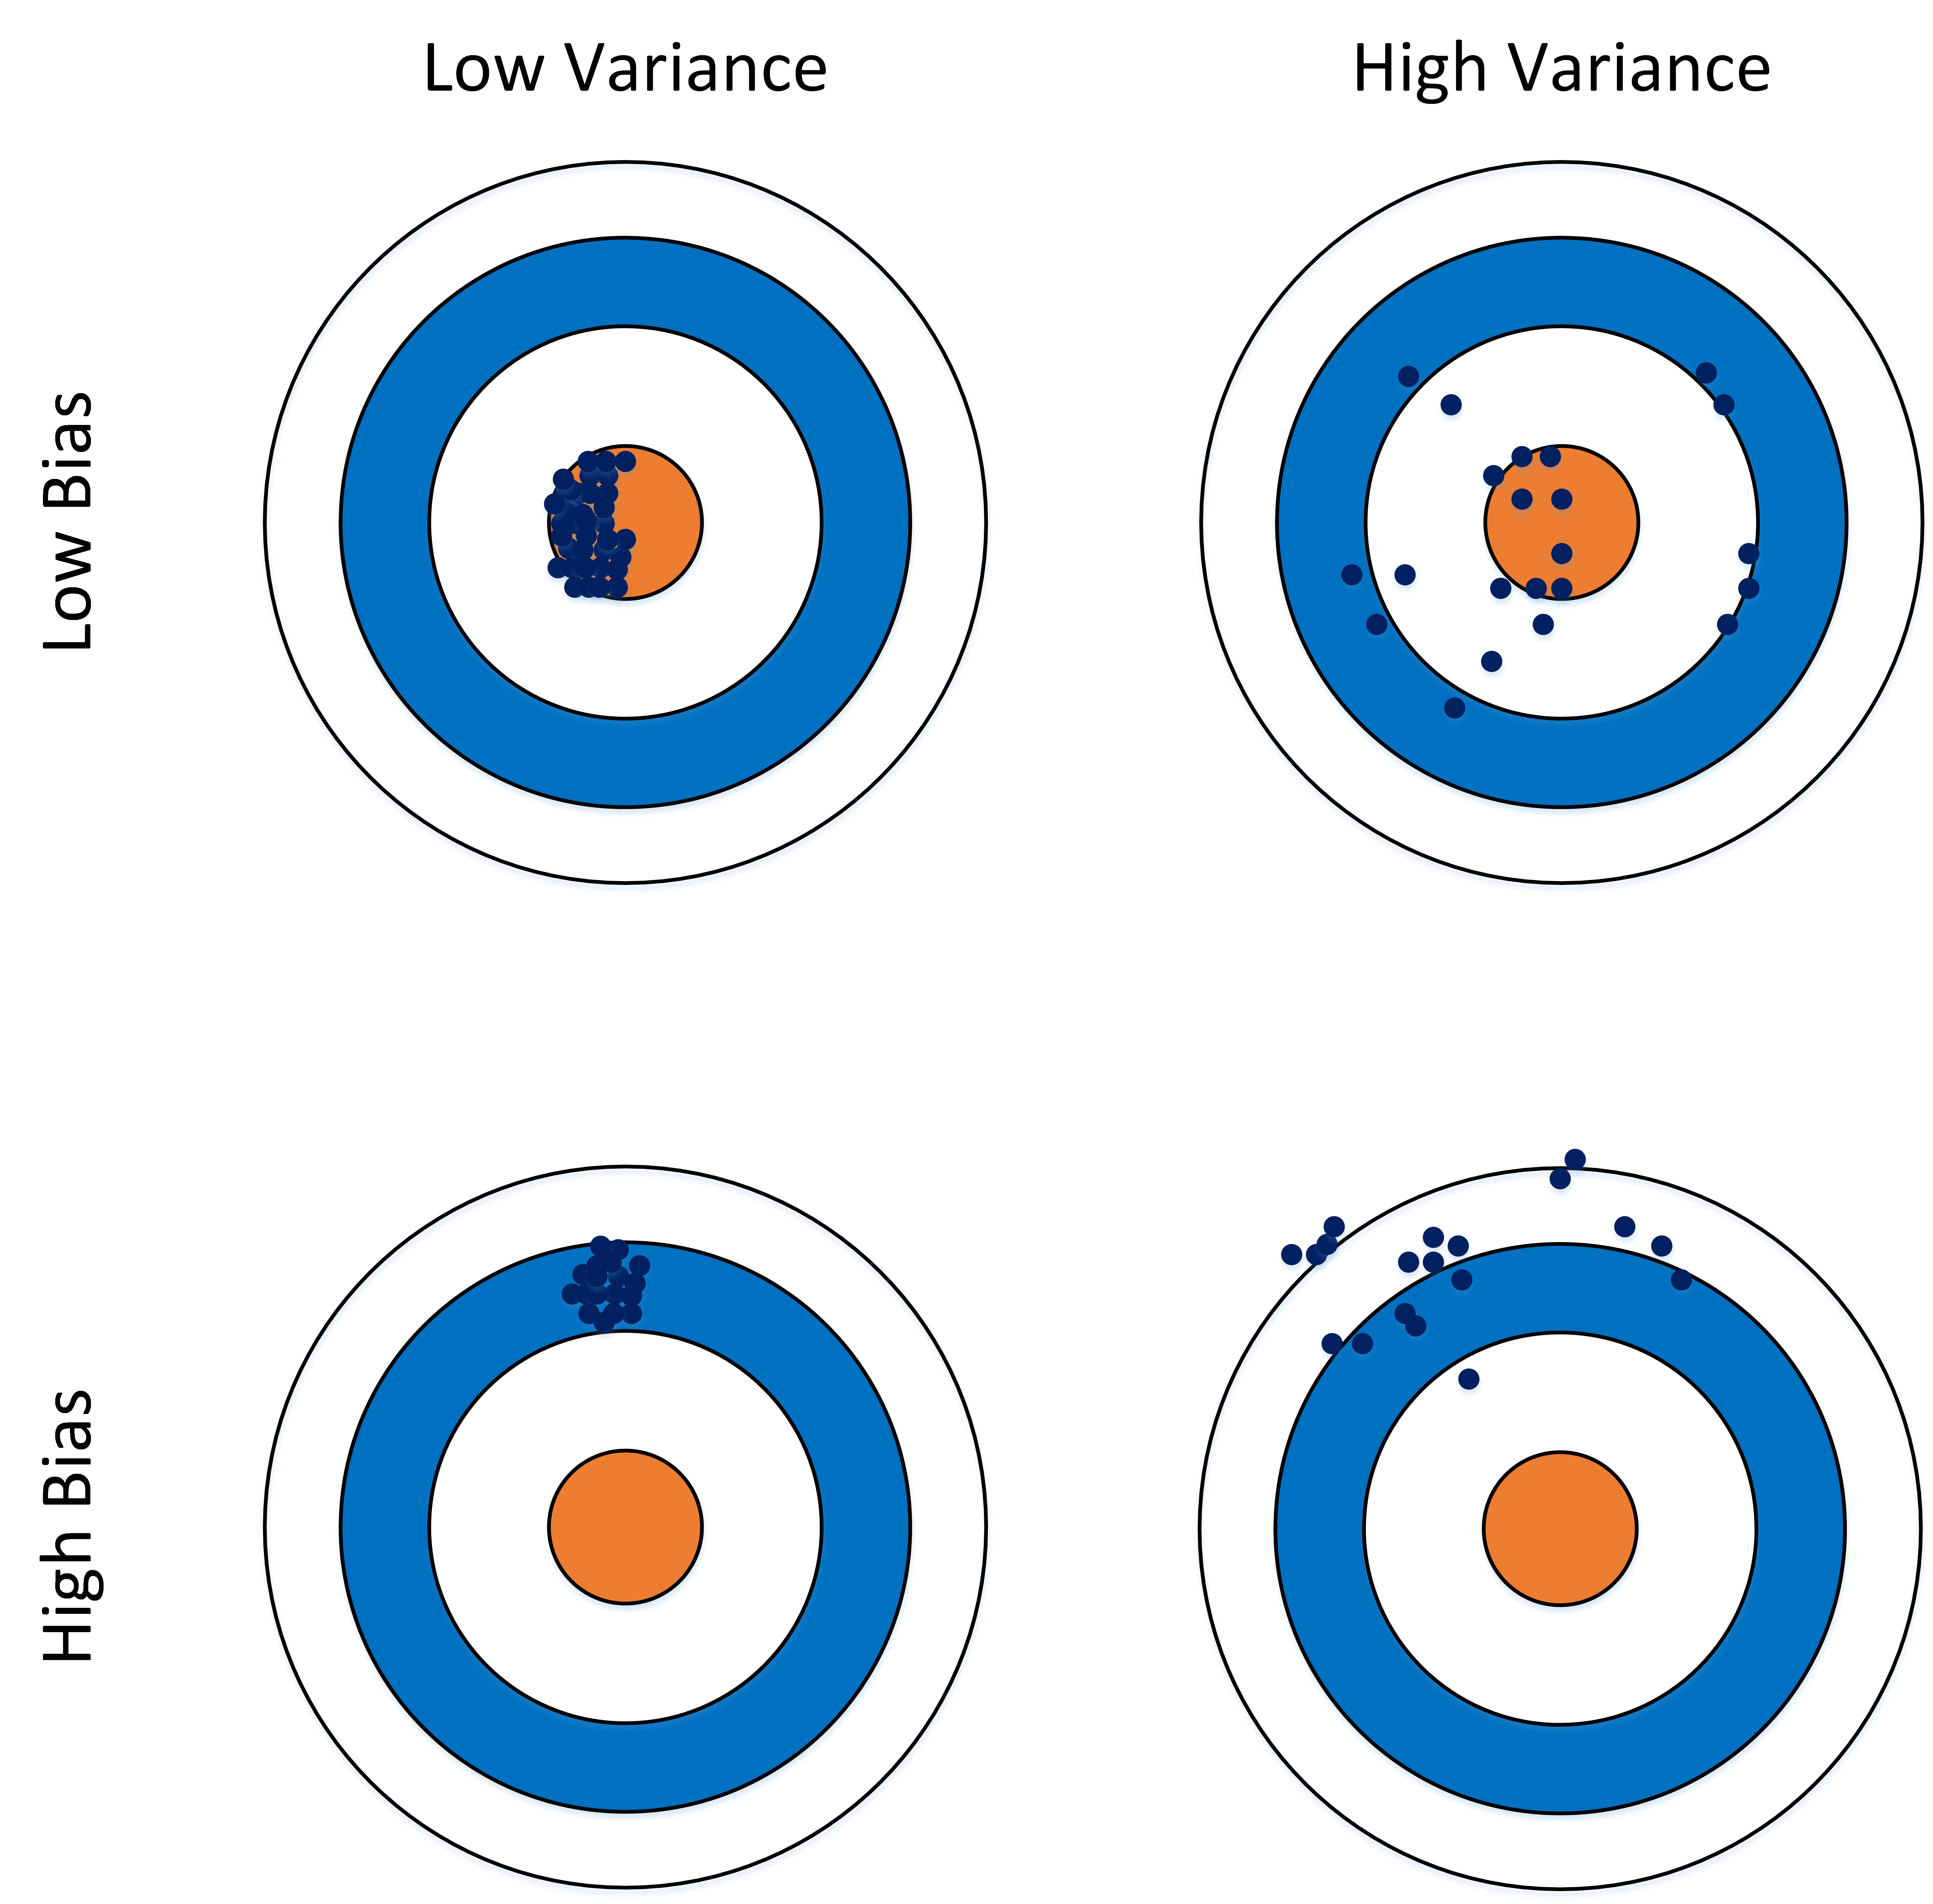
\includegraphics[width=0.5\textwidth]{figures/error1.png}
	\caption{方差和偏差对数据分布的影响}
	\label{error1}
\end{figure}


\subsection{损失函数}
\subsubsection{常见的损失函数}
损失函数可分为经验风险损失函数和结构风险损失函数。经验风险损失函数指预测结果和实际结果的差别,结构风险损失函数是在经验风险损失函数上加上正则项。
\paragraph{0-1损失函数}
$$L(Y, f(x)) =
\begin{cases}
1,& Y\ne f(x)\\
0,& Y = f(x)
\end{cases}$$
一般的在实际使用中,相等的条件过于严格,可适当放宽条件:
$$L(Y, f(x)) =
\begin{cases}
1,& |Y-f(x)| \geq T\\
0,& |Y-f(x)|< T
\end{cases}$$
\paragraph{绝对值损失函数}
$$L(Y, f(x)) = |Y-f(x)|​$$
\paragraph{平方损失函数}
$$L(Y, f(x)) = \sum_N{(Y-f(x))}^2$$
\paragraph{对数损失函数}
$$L(Y, P(Y|X)) = -\log{P(Y|X)}$$
常见的逻辑回归使用的就是对数损失函数,有很多人认为逻辑回归的损失函数是平方损失,其实不然。逻辑回归它假设样本服从伯努利分布(0-1分布),进而求得满足该分布的似然函数,接着取对数求极值等。逻辑回归推导出的经验风险函数是最小化负的似然函数,从损失函数的角度看,就是对数损失函数。
\paragraph{指数损失函数}
$$L(Y, f(x)) = \exp(-Yf(x))$$
\paragraph{Hinge损失函数}
$$L(y) = \max{(0, 1-ty)}$$
统一的形式:
$$L(Y, f(x)) = \max{(0, Yf(x))}$$
其中y是预测值,范围为(-1,1),t为目标值,其为-1或1。





\subsection{代价函数}
\subsubsection{为什么需要代价函数}
\begin{enumerate}
	\item 为了得到训练逻辑回归模型的参数,需要一个代价函数,通过训练代价函数来得到参数。
	\item 用于找到最优解的目的函数。
\end{enumerate}
\subsubsection{代价函数作用原理}
以平方误差代价函数为例,假设函数为$h(x)=\theta_0x$。平方误差代价函数的主要思想就是将实际数据给出的值与拟合出的线的对应值做差,求出拟合出的直线与实际的差距。在实际应用中,为了避免因个别极端数据产生的影响,采用类似方差再取二分之一的方式来减小个别数据的影响。因此,引出代价函数:
$$J(\theta_0, \theta_1) = \frac{1}{m}\sum_{i=1}^m(h(x^{(i)})-y^{(i)})^2$$
最优解即为代价函数的最小值$\min J(\theta_0, \theta_1)$。如果是1个参数,代价函数一般通过二维曲线便可直观看出。如果是2个参数,代价函数通过三维图像可看出效果,参数越多,越复杂。
当参数为2个时,代价函数是三维图像,如图\ref{costfunction1}所示。
\begin{figure}[htb]
	\centering
	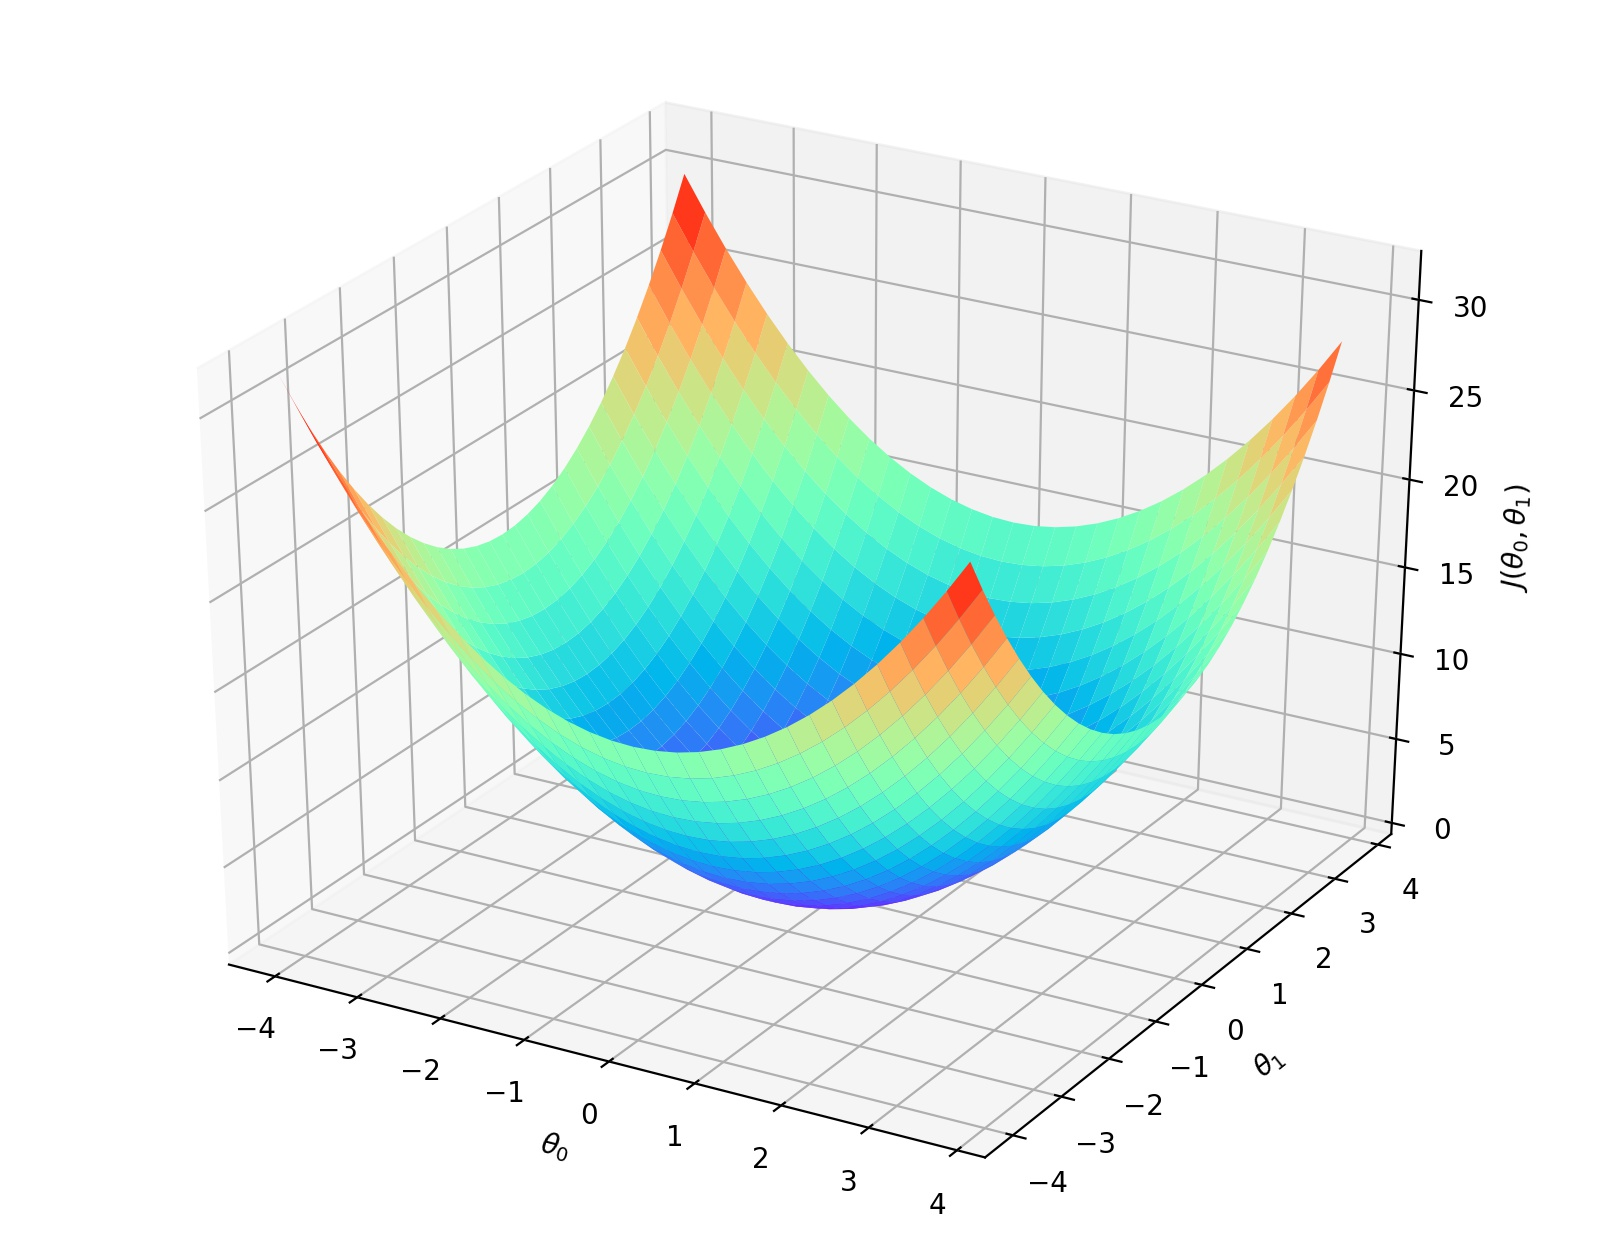
\includegraphics[width=0.5\textwidth]{figures/costfunction1.jpg}
	\caption{代价函数的三维图像}
	\label{costfunction1}
\end{figure}
\subsubsection{代价函数一定要非负吗?}
目标函数存在一个下界,在优化过程当中,如果优化算法能够使目标函数不断减小,根据单调有界准则,这个优化算法就能证明是收敛有效的。
\par 但是只要设计的目标函数有下界,基本上都可以,代价函数非负更为方便。
\subsubsection{常见的代价函数}
\paragraph{二次代价函数(quadratic cost)}
$$J = \frac{1}{2n}\sum_x\Vert y(x)-a^L(x)\Vert^2$$
其中,$J$表示代价函数,$x$表示样本,$y$表示实际值,$a$表示输出值,$n$表示样本的总数。使用一个样本为例简单说明,此时二次代价函数为:
$$J = \frac{(y-a)^2}{2}$$
假如使用梯度下降法(Gradient descent)来调整权值参数的大小,权值$w$和偏置$b$的梯度推导如下:
$$\frac{\partial J}{\partial b}=(a-y)\sigma'(z)$$
其中,$z​$表示神经元的输入,$\sigma​$表示激活函数。权值$w​$和偏置$b​$的梯度跟激活函数的梯度成正比,激活函数的梯度越大,权值$w​$和偏置$b​$的大小调整得越快,训练收敛得就越快。
\paragraph{交叉熵代价函数(cross-entropy)}
$$J = -\frac{1}{n}\sum_x[y\ln a + (1-y)\ln{(1-a)}]$$
其中,$J$表示代价函数,$x$表示样本,$y$表示实际值,$a$表示输出值,$n$表示样本的总数。
权值$w$和偏置$b​$的梯度推导如下:
$$\frac{\partial J}{\partial w_j}=\frac{1}{n}\sum_{x}x_j(\sigma{(z)}-y),\ 
\frac{\partial J}{\partial b}=\frac{1}{n}\sum_{x}(\sigma{(z)}-y)$$
当误差越大时,梯度就越大,权值$w$和偏置$b$调整就越快,训练的速度也就越快。
\subparagraph{将交叉熵看做是代价函数的两点原因}
\begin{itemize}
	\item 它是⾮负的, C > 0。可以看出:式子中的求和中的所有独⽴的项都是负数的,因为对数函数的定义域是(0,1),并且求和前⾯有⼀个负号,所以结果是非负。
	\item 如果对于所有的训练输⼊x,神经元实际的输出接近⽬标值,那么交叉熵将接近0。
\end{itemize}
\paragraph{对数似然代价函数(log-likelihood cost)}
对数似然函数常用来作为softmax回归的代价函数。深度学习中普遍的做法是将softmax作为最后一层,此时常用的代价函数是对数似然代价函数。
对数似然代价函数与softmax的组合和交叉熵与sigmoid函数的组合非常相似。对数似然代价函数在二分类时可以化简为交叉熵代价函数的形式。
\subsubsection{为什么用交叉熵代替二次代价函数}
\paragraph{为什么不用二次方代价函数}
由上一节可知,权值$w$和偏置$b$的偏导数为$\frac{\partial J}{\partial w}=(a-y)\sigma'(z)x$,$\frac{\partial J}{\partial b}=(a-y)\sigma'(z)$, 偏导数受激活函数的导数影响,sigmoid函数导数在输出接近0和1时非常小,会导致一些实例在刚开始训练时学习得非常慢。
\paragraph{为什么要用交叉熵}
交叉熵函数权值$w$和偏置$b$的梯度推导为:
$$\frac{\partial J}{\partial w_j}=\frac{1}{n}\sum_{x}x_j(\sigma{(z)}-y),\ 
\frac{\partial J}{\partial b}=\frac{1}{n}\sum_{x}(\sigma{(z)}-y)$$
由以上公式可知,权重学习的速度受到$\sigma{(z)}-y$影响,更大的误差,就有更快的学习速度,避免了二次代价函数方程中因$\sigma'{(z)}$导致的学习缓慢的情况。












\newpage
\section{神经网络}
\subsection{什么是神经网络}
\begin{itemize}
	\item 定义:具有适应性的简单单元组成的广泛并行互联的网络其组织能够模拟生物神经系统对真实世界物体所做出的交互反应
	\item 基础单位:神经元模型:兴奋——发送物质——引起相连神经元电位变化——达到阈值——激活——兴奋
	\item 组成: \begin{itemize}
		\item n个其他神经元的{\bfseries 输入信号}
		\item n个{\bfseries 带权重的连接}
		\item {\bfseries 阈值}
		\item {\bfseries 激活函数}及其产生的{\bfseries 输出}
	\end{itemize}
\end{itemize}

\subsection{为什么要用神经网络}
{\bfseries 仿生学}原理:{\bfseries 模仿人脑的结构},获得最好的表现

\subsection{神经网络怎么训练}
\subsubsection{成本函数的建立}
神经网络,乃至于一切机器学习模型,究竟应该如何训练呢?
\par
根据(愚蠢的)人类的经验,我们都是先照猫画虎,照着别人做,随后在犯错误后被家长或老师或其他长辈训斥,从而获得经验,改变提高自己,从而提升自己的能力的。
\par
人类试图将自己的学习过程(并不怎么聪明和有效率)应用到一切机器学习模型(因此也包括神经网络)上。
\par
其中最重要的(之一),同时也是必须最先做的工作,就是找到告诉机器它做错了的办法。就像当初我们挨打或者挨骂那样,告诉机器应该改正自己的行为了。
\par
于是,数学家们就想到了,用一个函数来表示犯错成本,这个函数值越大,说明机器做错的事情越多,错误的程度越严重,以此来对命令机器进行反思,改进,最后在这方面表现的更好(也就是函数值更低)。
\par
所以,首先,我们需要量化一个指标来对神经网络的表现进行评价和测量,以此作为标准对神经网络的参数进行优化。这就是成本函数。
\begin{enumerate}
	\item 首先确立建立模型时想要{\bfseries 最大化的可能性}$L$,假设样本个体都{\bfseries 相互独立},则有假设: $$L(\pmb w)=P(y|\pmb x;\pmb w) = \prod_{i=1}^nP(y^{(i)} | \pmb x^{(i)};\pmb w)=\prod_{i=1}^n(\phi(z^{(i)}))^{y^{(i)}}((1-\phi(z^{(i)}))^{1-y^{(i)}}$$
	\item 求得该函数的{\bfseries 对数似然函数}为: $$l(\pmb w) = \log(L(\pmb w)) = \sum_{i=1}^n[y^{(i)}\log(\phi(z^{(i)})) + (1-y^{(i)})\log(1-\phi(z^{(i)}))]$$
	\item 用{\bfseries 梯度下降法最小化代价函数}$J$可得: $$J(\pmb w) = -\sum_{i=1}^ny^{[i]}\log(a^{[i]}) + (1-y^{[i]})\log(1-a^{[i]})$$ \begin{itemize}
		\item 其中 $y^{[i]} = \phi(z^{[i]})$:数据集中{\bfseries 第i个样本}用前向传播算法计算出的Sigmoid值
		\item 其中上标 $i$ 为训练集中{\bfseries 特定样本}的索引
	\end{itemize}
	\item {\bfseries 添加正则化项减少过拟合机会}: $$L2 = \lambda \|\pmb w\|_2^2 = \lambda\sum_{j=1}^mw_j^2$$ \begin{itemize}
		\item 其中 $j$ 是{\bfseries 某一种特征}
	\end{itemize}
	\item {\bfseries 综合以上两者可得}: $$J(\pmb w) = -[\sum_{i=1}^ny^{[i]}\log(a^{[i]}) + (1-y^{[i]})\log(1-a^{[i]})] + \frac{\lambda}{2}\|\pmb w\|_2^2$$
\end{enumerate}

\subsubsection{多元分类MLP的逻辑成本函数}
\begin{itemize}
	\item 对于用于多元分类的MLP,返回的是一个有$t${\bfseries 个元素的输出向量},需要与$t*1${\bfseries 维独热编码表示的向量}进行比较:
	$$\pmb a^{(out)} = \begin{bmatrix}0.1 \\ 0.9 \\ ... \\ 0.3 \end{bmatrix},\ y = \begin{bmatrix}0 \\ 1 \\ ... \\ 0 \end{bmatrix}$$
	\item 将逻辑成本函数推广到网络中{\bfseries 所有的t激活单元},可得{\bfseries 成本函数}({\bfseries 不包括正则化项})为: 
	$$J(\pmb W) = - \sum_{i=1}^n\sum_{j=1}^ty_j^{[i]}\log(\pmb a^{[i]}_j) + (1-y_j^{[i]})\log(1-\pmb a^{[i]}_j)$$ \begin{itemize}
		\item 其中上标 $i$ 为训练集中特定样本的索引
		\item 其中下标 $j$ 为某一种特征
	\end{itemize}
	\item {\bfseries 惩罚项}为:
	$$\frac{\lambda}{2}\sum_{l=1}^{L-1}\sum_{i=1}^{u_l}\sum_{i=1}^{u_{l+1}}(w_{j,i}^{(l)})^2$$ \begin{itemize}
		\item 其中 $u_l$ 是一个给定的1层单位数
	\end{itemize}
	\item {\bfseries 综上可得}:$$J(\pmb W) = - \sum_{i=1}^n\sum_{j=1}^ty_j^{[i]}\log(\pmb a^{[i]}_j) + (1-y_j^{[i]})\log(1-\pmb a^{[i]}_j) + \frac{\lambda}{2}\sum_{l=1}^{L-1}\sum_{i=1}^{u_l}\sum_{i=1}^{u_{l+1}}(w_{j,i}^{(l)})^2$$
\end{itemize}

\subsubsection{反向传播算法}
\paragraph{为什么不用正向传播算法?}
答案其实很简单。因为正向传播算法做的是矩阵和矩阵的乘法,而反向传播算法做的是矩阵和向量的乘法,会节省很多计算资源。
\paragraph{适用范围}
多层前馈神经网络和其他神经网络。
\paragraph{关键思想}
{\bfseries 从后往前,层层求导}
\paragraph{神经网络组成}
在此我们先规定一下神经网络的各个部分及其符号,利于我们之后讨论参数更新等问题。
\begin{itemize}
	\item {\bfseries 输入层} \emph{d}个输入:接收输入$x_i$
	\item {\bfseries 隐含层} \emph{q}个神经元:接收输入$\alpha_h = \sum_{i=1}^dv_{ih}x_i$,其中$v_{ih}$为权重,输入经过激活函数以后和阈值$\gamma_h$进行比较,输出为$b_h$
	\item {\bfseries 输出层} \emph{l}个神经元:接收输入$\beta_j = \sum_{h=1}^qw_{hj}b_h$,其中$w_{hj}$为权重,输入经过激活函数以后和阈值$\theta_j$进行比较,输出为$y_i$
\end{itemize}
\par
其中,一般{\bfseries 输入个数为参数个数,输出个数为标记个数}
\par
{\bfseries 参数个数}:$d*q$个权重$+q$个阈值$+q*l$个权重$+l$个阈值
\paragraph{输出}
假定$\hat{\pmb {y}_k} = (\hat{y_1^k}, \hat{y_2^k}, ..., \hat{y_l^k})$,其中$\hat{y_j^k} = f(\beta_j - \theta_j)$
\paragraph{优化目标:均方误差}
对第k个样例求所有l个属性值的均方误差。1/2求导时使用:$$E_k = \frac{1}{2}\sum_{j=1}^l(\hat{y}_j^k - {y_j^k})$$
\paragraph{激活函数}
假设隐层和输出层神经元都是用Sigmoid函数(实际上是对数函数)

\subsubsection{参数更新方法(以隐层到输出层的连接权$w_{hj}$为例)}
\paragraph{策略:梯度下降}
以目标的的负梯度方向进行参数调整
\paragraph{一句话方法}
对均方误差$E_k$和学习率$\eta$求第二层权重的改变量
\paragraph{均方误差对权重求导的过程}
\subparagraph{总目标}
$\varDelta w_{hj} = -\eta \frac{\partial E_k}{\partial w_{hj}}$
\subparagraph{推导过程}
\begin{enumerate}
	\item 由{\bfseries 链式求导法则}可得:$$\frac{\partial E_k}{\partial w_{hj}} = \frac{\partial E_k}{\partial \hat{y}_j^k} \cdot \frac{\partial \hat{y}_j^k}{\partial \beta_j} \cdot \frac{\partial \beta_j}{\partial w_{hj}}$$
	\item 根据$\beta_j$的{\bfseries 定义}可得:$$\frac{\partial \beta_j}{\partial w_{hj}} = b_h$$
	\item Sigmoid函数的性质:$$f'(x) = f(x)(1 - f(x))$$
	\item 根据定义:$$f(\beta_j - \theta_j) = \hat{y_j^k}$$
	\item 由2,3,4可得{\bfseries 输出层神经网络的梯度项}:$$\begin{aligned} \pmb g_j &= -\frac{\partial E_k}{\partial \hat{y}_j^k} \cdot \frac{\partial \hat{y}_j^k}{\partial \beta_j} \\ &= -(\hat{y}_j^k - {y_j^k})f'(\beta_j - \theta_j) \qquad (a) \\ &= \hat{y}_j^k(1 - \hat{y}_j^k)({y_j^k} - \hat{y}_j^k) \qquad (b) \end{aligned}$$ \begin{enumerate}
		\item 各自求导
		\item Sigmoid函数的性质
	\end{enumerate}
	\item 综上所述,可得:$$\varDelta w_{hj} = \eta\pmb g_jb_h$$ $$\varDelta\theta_j = -\eta\pmb g_j$$
	\item 类似可得{\bfseries 隐含层神经网络的梯度项}:$$\begin{aligned} e_h &= - \frac{\partial E_k}{\partial b_h} \cdot \frac{\partial b_h}{\partial a_h} \\ & = -\sum_{j=1}^l \frac{\partial E_k}{\partial \beta_j} \cdot \frac{\partial \beta_j}{\partial b_h} f'(a_h-\gamma_h) \qquad (a)\\ & = \sum_{j=1}^lw_{hj}\pmb g_j f'(a_h - \gamma_h)\qquad (b) \\ & = b_h(1 - b_h)\sum_{j=1}^lw_{hj}\pmb g_j \qquad (c) \end{aligned}$$ \begin{enumerate}
		\item 利用上一层的梯度项
		\item 将$\pmb g_j$代入
		\item Sigmoid函数的性质
	\end{enumerate}
	\item 综上所述可得:$$\varDelta v_{ih} = \eta\pmb e_hx_i$$
	$$\varDelta\theta_j = -\eta\pmb e_h$$
\end{enumerate}
\paragraph{结果分析}
\subparagraph{$\varDelta w_{hj} = \eta\pmb g_jb_h$ }
和下层的权重$\pmb g_j$和本层的输出$b_h$有关
\subparagraph{$\varDelta\theta_j = -\eta\pmb g_j$}
本层的阈值只和梯度项有关
\subparagraph{$\varDelta v_{ih} = \eta\pmb e_hx_i$}
类似
\subparagraph{$\varDelta\theta_j = -\eta\pmb e_h$}
类似

\subsubsection{算法流程}
\paragraph{输入}
\begin{itemize}
	\item 将输入示例提供给输入层神经元
	\item 逐层将信号向前传
	\item 产生输出层的结果$y_j^k$
\end{itemize}
\paragraph{迭代}
\begin{itemize}
	\item 计算输出层的误差$\pmb g_j$
	\item 将误差逆向传播至隐层神经元$\pmb e_h$
	\item 根据隐层神经元的误差来对连接权和阈值进行调整 \begin{itemize}
		\item 更新阈值 \begin{itemize}
			\item $\varDelta\theta_j = -\eta\pmb g_j$
			\item $\varDelta\theta_j = -\eta\pmb e_h$
		\end{itemize}
		\item 更新权重 \begin{itemize}
			\item $\varDelta w_{hj} = \eta\pmb g_jb_h$
			\item $\varDelta v_{ih} = \eta\pmb e_hx_i$
		\end{itemize}
	\end{itemize}
\end{itemize}
\paragraph{判断当前的累积误差是否已经足够小}
$E = \frac{1}{m}\sum_{k=1}^mE_k$ (其中$E_k$为单个样本的均方误差)

\begin{algorithm}[htb]  
	\caption{反向传播算法}  
	\begin{algorithmic}[1]  
	  \Require  
	  	$训练集D = \{(\pmb x_k, \pmb y_k)\}_{k=1}^m$,学习率$\eta$  
	  \Ensure  
	  	连接权与阈值确定的多层前馈神经网络
	\While {没达到停止条件}  
		\ForAll {$(\pmb x_k, \pmb y_k)$属于集合D}
			\State 计算输出层的误差,
			根据当前参数和式计算当前样本的输出yk,
			计算输出层神经元的梯度项gj
  
			\State 将误差逆向传播至隐层神经元,
				计算隐层神经元的梯度项eh
		
			\State 更新连接权和阈值
		\EndFor;  
	\EndWhile  
	\\
	\Return $E_n$;  
	\end{algorithmic}  
\end{algorithm}  

\subsubsection{算法分类}
\paragraph{标准BP算法}
\begin{itemize}
	\item 优化目标:均方误差$E_k$
	\item 更新参数的单位:每一个样例进行一次
	\item 可能出现抵消效果
\end{itemize}
\paragraph{累计BP算法}
\begin{itemize}
	\item 优化目标:累积误差
	\item 更新参数的单位:针对整个训练集
	\item 到了一定迭代次数后进一步下降很缓慢,不如标准快
\end{itemize}

\subsubsection{过拟合针对}
\paragraph{早停}
\begin{itemize}
	\item 将数据分成训练集和验证集
    \item 训练集用来计算梯度、更新连接权和阈值
    \item 验证集用来估计误差
    \item 若训练误差降低但验证误差升高,则停止训练直接返回
\end{itemize}
\paragraph{正则化}
\begin{itemize}
	\item 基本思想:在误差目标函数中增加一个用于描述网络复杂度的部分
	\item 例如:连接权与阈值的平方和
	\item 取$\omega_i$表示连接权和阈值,则误差目标函数改变为:
	$$E = \lambda\frac{1}{m}\sum_{k=1}^mE_k + (1-\lambda)\sum_i\omega_i^2$$ \begin{itemize}
		\item $\lambda$取值为$(0,1)$
		\item 用于对经验误差和网络复杂度这两项进行折中,通过交叉验证法来估计
	\end{itemize}
\end{itemize}

\subsubsection{参数优化}
\paragraph{目标}
累计误差最小,是关于$\omega$和$\theta$的函数,全局最小
\paragraph{相关概念}
\begin{itemize}
	\item 局部最小:邻域中最小
	\item 全局最小:整个参数空间中最小
	\item 负梯度方向:函数值下降最快的方向
	\item 当梯度项为0时,达到局部最小,并停止更新
\end{itemize}
\paragraph{问题}
可能有多个局部最小,避免参数最优陷入局部最小
\paragraph{跳出局部极小}
\begin{itemize}
	\item 以多组不同的参数值初始化,取其中误差最小的参数
	\item 模拟退火:每一步都以一定概率接受次优解。并且这个概率随着时间的推移而逐渐降低,以保证算法稳定
	\item 使用随机梯度下降:在计算梯度下降时加入随机因素
	\item 遗传算法
\end{itemize}

\subsection{超参数}
\subsubsection{定义}
在机器学习的上下文中,超参数是在开始学习过程之前设置值的参数,而不是通过训练得到的参数数据。通常情况下,需要对超参数进行优化,给学习机选择一组最优超参数,以提高学习的性能和效果。
\paragraph{常见存在于}
\begin{enumerate}
	\item 定义关于模型的更高层次的概念,如复杂性或学习能力。
	\item 不能直接从标准模型培训过程中的数据中学习,需要预先定义。
	\item 可以通过设置不同的值,训练不同的模型和选择更好的测试值来决定。
\end{enumerate}
\paragraph{具体实例}
算法中的学习率(learning rate)、梯度下降法迭代的数量(iterations)、隐藏层数目(hidden layers)、隐藏层单元数目、激活函数( activation function)都需要根据实际情况来设置,这些数字实际上控制了最后的参数和的值,所以它们被称作超参数。
\subsubsection{设置方法}
\begin{enumerate}
	\item 猜测和检查:根据经验或直觉,选择参数,一直迭代。
	\item 网格搜索:让计算机尝试在一定范围内均匀分布的一组值。
	\item 随机搜索:让计算机随机挑选一组值。
	\item 贝叶斯优化:使用贝叶斯优化超参数,会遇到贝叶斯优化算法本身就需要很多的参数的困难。
	\item MITIE方法,好初始猜测的前提下进行局部优化。它使用BOBYQA算法,并有一个精心选择的起始点。由于BOBYQA只寻找最近的局部最优解,所以这个方法是否成功很大程度上取决于是否有一个好的起点。在MITIE的情况下,我们知道一个好的起点,但这不是一个普遍的解决方案,因为通常你不会知道好的起点在哪里。从好的方面来说,这种方法非常适合寻找局部最优解。
	\item LIPO的全局优化方法。这个方法没有参数,而且经验证比随机搜索方法好。
\end{enumerate}
\subsubsection{超参数搜索一般过程}
\begin{enumerate}
	\item 将数据集划分成训练集、验证集及测试集。
	\item 在训练集上根据模型的性能指标对模型参数进行优化。
	\item 在验证集上根据模型的性能指标对模型的超参数进行搜索。
	\item 步骤2和步骤3交替迭代,最终确定模型的参数和超参数,在测试集中验证评价模型的优劣。
\end{enumerate}

\subsection{激活函数}
\subsubsection{问题}
\begin{enumerate}
	\item 线性神经网络无法解决非线性问题。
	\item 需要一个函数可以对得到的Y值进行分类。
	\item 如果输入的绝对值特别大,或者无限大,那么输出就会特别大,直接导致error太大。更新出来的权值没有意义,或者无法更新权值。
	\item 反向传播的时候线性的导数是常数,导致无法继续传播。
\end{enumerate}
\subsubsection{常用激活函数}
如图\ref{activationfunction1}所示。除此以外还有SoftMax,SoftPlus等等。
\begin{figure}[htb]
	\centering
	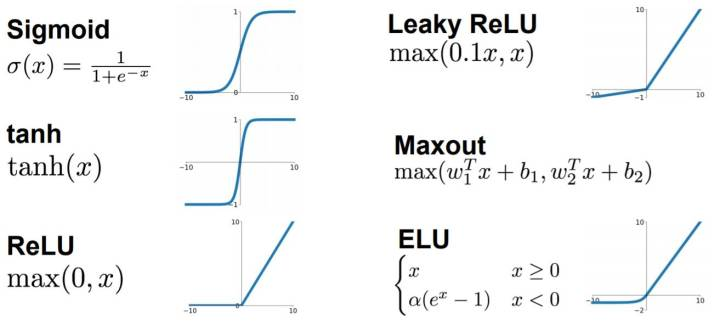
\includegraphics[width=1.0\textwidth]{figures/activationfunction1.jpg}
	\caption{常见激活函数}
	\label{activationfunction1}
\end{figure}
\subsubsection{作用}
\begin{itemize}
	\item 提高模型鲁棒性
	\item 提高模型非线性表达能力
	\item 缓解梯度消失问题
	\item 将特征图映射到新的特征空间从何更有利于训练
	\item 加速模型收敛
\end{itemize}
\subsubsection{常见激活函数的导数计算}
\begin{itemize}
	\item Sigmoid激活函数 \begin{itemize}
		\item 函数表达式:$f(x)=\frac{1}{1+e^{-x}}$
		\item 导数:$f^{'}(x)=\frac{1}{1+e^{-x}}\left( 1- \frac{1}{1+e^{-x}} \right)=f(x)(1-f(x))$
		\item 备注:当$x=10$,或$x=-10$,$f^{'}(x) \approx0$,当$x=0$,$f^{'}(x) =0.25$
	\end{itemize}
	\item Tanh激活函数 \begin{itemize}
		\item 函数表达式:$f(x)=tanh(x)=\frac{e^x-e^{-x}}{e^x+e^{-x}}$
		\item 导数:$f^{'}(x)=-(tanh(x))^2$
		\item 备注:当$x=10$,或$x=-10$,$f^{'}(x) \approx0$,当$x=0$,$f^{`}(x) =1$
	\end{itemize}
	\item Relu激活函数 \begin{itemize}
		\item 函数表达式:$f(x)=max(0,x)$
		\item 导数:$c(u)=\begin{cases} 0,x<0 \\ 1,x>0 \\ undefined,x=0\end{cases}$
		\item 备注:通常$x=0$时,给定其导数为1和0
	\end{itemize}
\end{itemize}
\subsubsection{激活函数性质}
\begin{itemize}
	\item 非线性: 当激活函数是线性的,一个两层的神经网络就可以基本上逼近所有的函数。但如果激活函数是恒等激活函数的时候,即 $ f(x)=x $,就不满足这个性质,而且如果 MLP 使用的是恒等激活函数,那么其实整个网络跟单层神经网络是等价的
	\item 可微性: 当优化方法是基于梯度的时候,就体现了该性质
	\item 单调性: 当激活函数是单调的时候,单层网络能够保证是凸函数
	\item $f(x) \approx x$: 当激活函数满足这个性质的时候,如果参数的初始化是随机的较小值,那么神经网络的训练将会很高效;如果不满足这个性质,那么就需要详细地去设置初始值
	\item 输出值的范围: 当激活函数输出值是有限的时候,基于梯度的优化方法会更加稳定,因为特征的表示受有限权值的影响更显著;当激活函数的输出是无限的时候,模型的训练会更加高效,不过在这种情况小,一般需要更小的 Learning Rate。
\end{itemize}
\subsubsection{选择激活函数的策略}
选择一个适合的激活函数并不容易,需要考虑很多因素,通常的做法是,如果不确定哪一个激活函数效果更好,可以把它们都试试,然后在验证集或者测试集上进行评价。然后看哪一种表现的更好,就去使用它。
\begin{itemize}
	\item 如果输出是0、1值(二分类问题),则输出层选择sigmoid函数,然后其它的所有单元都选择Relu函数。
	\item 如果在隐藏层上不确定使用哪个激活函数,那么通常会使用Relu激活函数。有时,也会使用 tanh 激活函数,但Relu的一个优点是:当是负值的时候,导数等于0。
	\item sigmoid激活函数:除了输出层是一个二分类问题基本不会用它。
	\item tanh激活函数:tanh是非常优秀的,几乎适合所有场合。
	\item ReLu激活函数:最常用的默认函数,如果不确定用哪个激活函数,就使用ReLu或者Leaky ReLu,再去尝试其他的激活函数。
	\item 如果遇到了一些死的神经元,我们可以使用Leaky ReLU函数。
\end{itemize}
\subsubsection{ReLu激活函数的优点}
\begin{itemize}
	\item 在区间变动很大的情况下,ReLu激活函数的导数或者激活函数的斜率都会远大于0,在实践中,使用ReLu激活函数神经网络通常会比使用sigmoid或者tanh激活函数学习的更快。
	\item sigmoid和tanh函数的导数在正负饱和区的梯度都会接近于0,这会造成梯度弥散,而Relu和Leaky ReLu函数大于0部分都为常数,不会产生梯度弥散现象。
	\item 需注意,Relu进入负半区的时候,梯度为0,神经元此时不会训练,产生所谓的稀疏性,而Leaky ReLu不会产生这个问题。
\end{itemize}
\subsubsection{Softmax函数}
\paragraph{定义}
$$P(i) = \frac{exp( \theta_i^T x)}{\sum_{k=1}^{K} exp(\theta_i^T x)}$$
其中,$\theta_i$和$x$是列向量,$\theta_i^T x $可能被换成函数关于$x$的函数$f_i(x)$。
通过Softmax函数,可以使得$ P(i) $的范围在$[0,1]$之间。在回归和分类问题中,通常 $ \theta $ 是待求参数,通过寻找使得$P(i)$最大的$\theta_i$作为最佳参数。
\paragraph{$e$的幂函数的意义}
参考logistic函数:
$$P(i) = \frac{1}{1+exp(-\theta_i^T x)}$$
这个函数的作用就是使得$P(i)$在负无穷到0的区间趋向于0, 在0到正无穷的区间趋向1。同样Softmax函数加入了$e$的幂函数正是为了两极化:正样本的结果将趋近于1,而负样本的结果趋近于0。这样为多类别提供了方便(可以把$ P(i) $看做是样本属于类别的概率)。可以说,Softmax函数是logistic函数的一种泛化。

\subsection{Batch Size}
\subsubsection{为什么需要Batch Size}
Batch的选择,首先决定的是下降的方向。如果数据集比较小,可采用全数据集的形式,好处是:
\begin{itemize}
	\item 由全数据集确定的方向能够更好地代表样本总体,从而更准确地朝向极值所在的方向。
	\item 由于不同权重的梯度值差别巨大,因此选取一个全局的学习率很困难。Full Batch Learning可以使用Rprop只基于梯度符号并且针对性单独更新各权值。
\end{itemize}
对于更大的数据集,假如采用全数据集的形式,坏处是:
\begin{itemize}
	\item 随着数据集的海量增长和内存限制,一次性载入所有的数据进来变得越来越不可行。
	\item 以Rprop的方式迭代,会由于各个Batch之间的采样差异性,各次梯度修正值相互抵消,无法修正。这才有了后来RMSProp的妥协方案。 
\end{itemize}
\subsubsection{Batch Size值的选择}
可采用批梯度下降法(Mini-batches Learning)。因为如果数据集足够充分,那么用一半(甚至少得多)的数据训练算出来的梯度与用全部数据训练出来的梯度是几乎一样的。
\subsubsection{增大Batch Size的好处}
\begin{enumerate}
	\item 内存利用率提高了,大矩阵乘法的并行化效率提高。
	\item 跑完一次epoch(全数据集)所需的迭代次数减少,对于相同数据量的处理速度进一步加快。
	\item 在一定范围内,一般来说batch size越大,其确定的下降方向越准,引起训练震荡越小。
\end{enumerate}
\subsubsection{盲目增大Batch Size的坏处}
\begin{itemize}
	\item 内存利用率提高了,但是内存容量可能撑不住了。
	\item 跑完一次epoch(全数据集)所需的迭代次数减少,要想达到相同的精度,其所花费的时间大大增加了,从而对参数的修正也就显得更加缓慢。
	\item batch size增大到一定程度,其确定的下降方向已经基本不再变化。
\end{itemize}

\subsection{归一化}
\subsubsection{归一化含义}
\begin{itemize}
	\item 归纳统一样本的统计分布性。归一化在$0-1$之间是统计的概率分布,归一化在$-1--+1$之间是统计的坐标分布.
	\item 无论是为了建模还是为了计算,首先基本度量单位要同一,神经网络是以样本在事件中的统计分别几率来进行训练(概率计算)和预测,且sigmoid函数的取值是0到1之间的,网络最后一个节点的输出也是如此,所以经常要对样本的输出归一化处理。
	\item 归一化是统一在$ 0-1 $之间的统计概率分布,当所有样本的输入信号都为正值时,与第一隐含层神经元相连的权值只能同时增加或减小,从而导致学习速度很慢。
	\item 另外在数据中常存在奇异样本数据,奇异样本数据存在所引起的网络训练时间增加,并可能引起网络无法收敛。为了避免出现这种情况及后面数据处理的方便,加快网络学习速度,可以对输入信号进行归一化,使得所有样本的输入信号其均值接近于0或与其均方差相比很小。
\end{itemize}
\subsubsection{归一化好处}
\begin{itemize}
	\item 为了后面数据处理的方便,归一化的确可以避免一些不必要的数值问题。
	\item 为了程序运行时收敛加快。
	\item 同一量纲。样本数据的评价标准不一样,需要对其量纲化,统一评价标准。这算是应用层面的需求。
	\item 避免神经元饱和。啥意思?就是当神经元的激活在接近 0 或者 1 时会饱和,在这些区域,梯度几乎为 0,这样,在反向传播过程中,局部梯度就会接近 0,这会有效地“杀死”梯度。
	\item 保证输出数据中数值小的不被吞食。 
\end{itemize}
\subsubsection{归一化能提高求解最优解速度的理由}
\begin{figure}[htb]
	\centering
	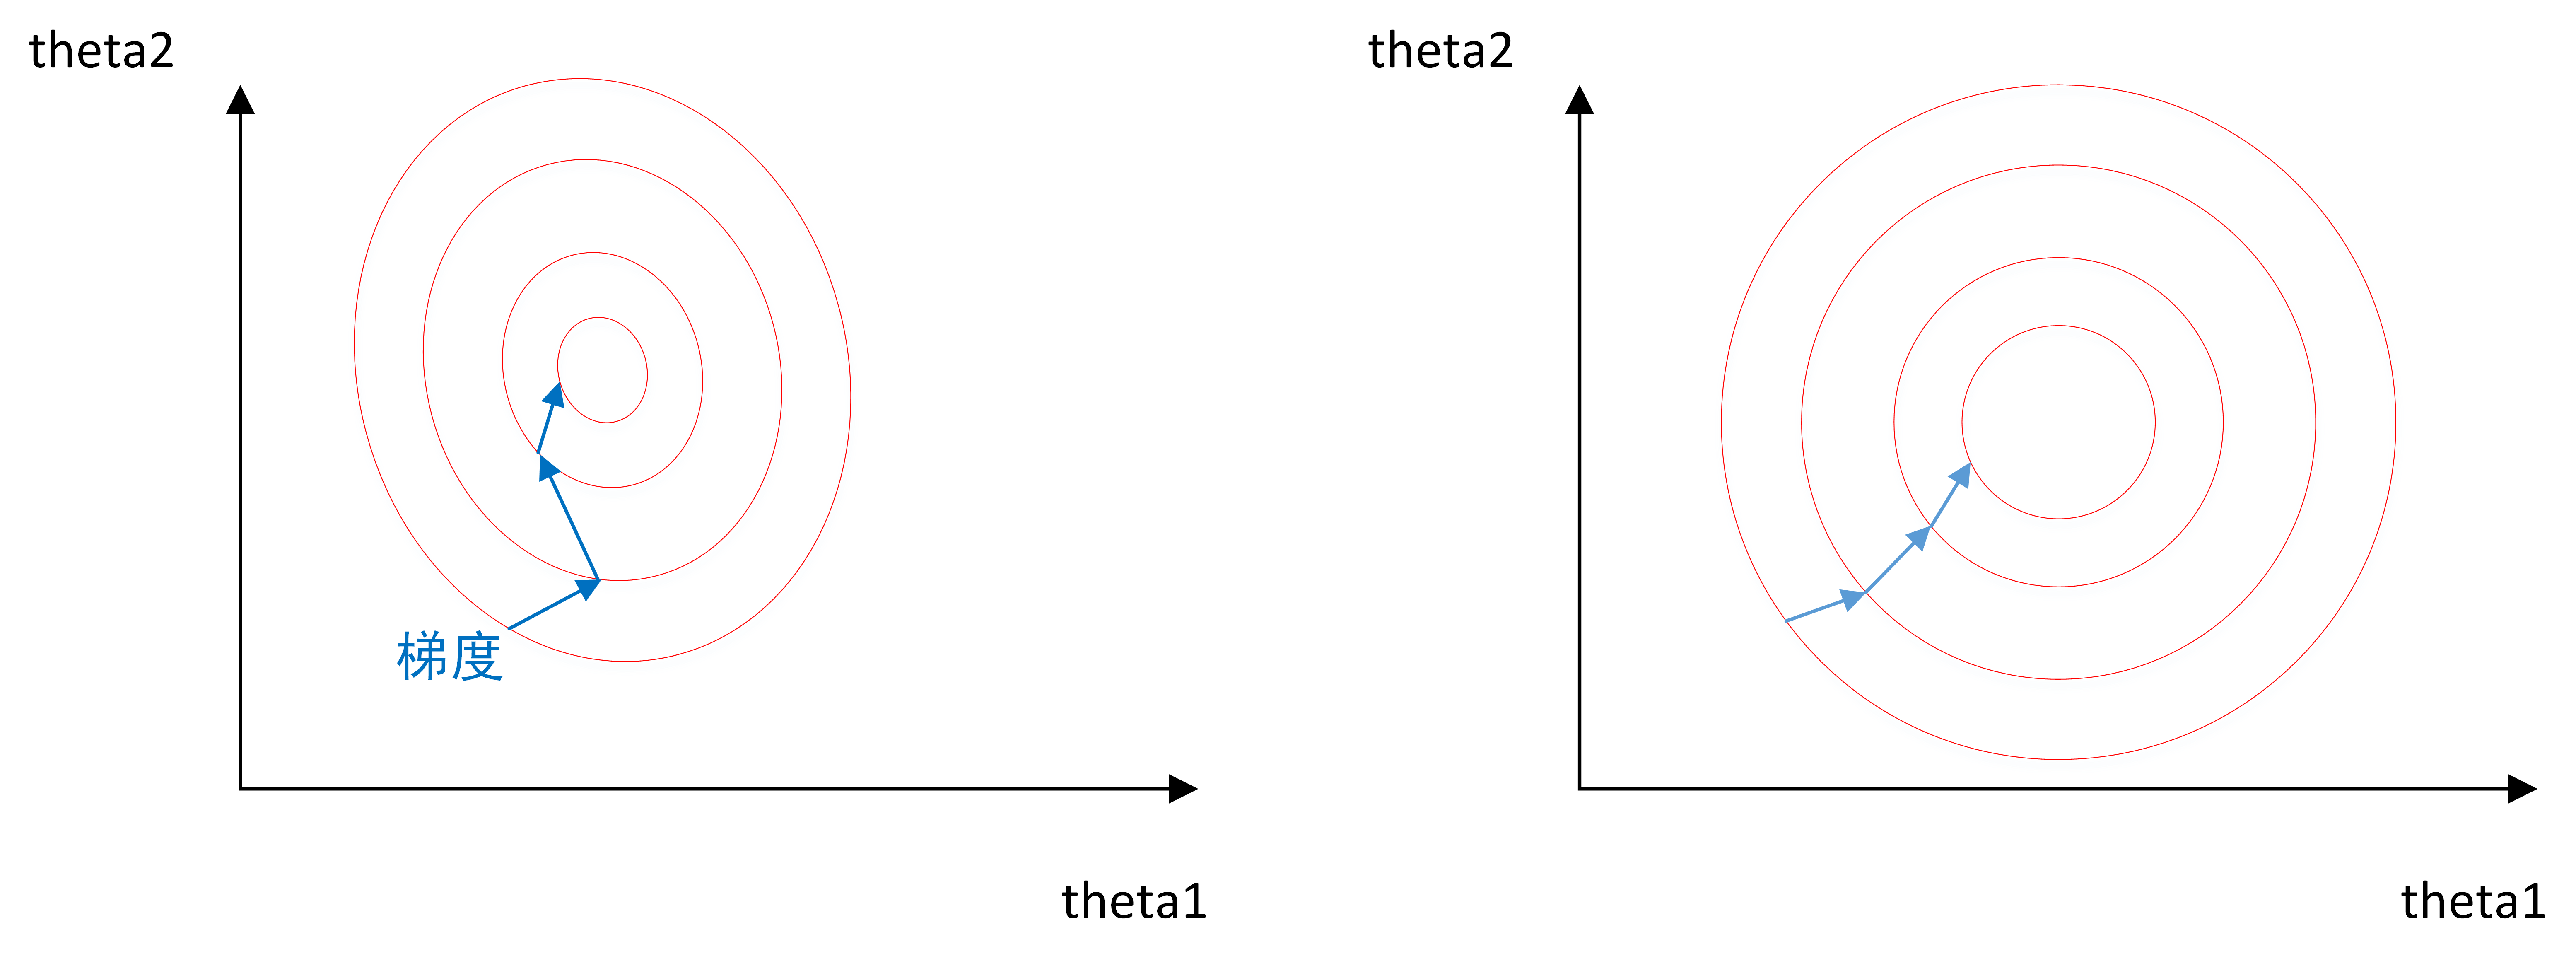
\includegraphics[width=0.5\textwidth]{figures/normalization1.png}
	\caption{归一化图示}
	\label{normalization1}
\end{figure}
上图是代表数据是否均一化的最优解寻解过程(圆圈可以理解为等高线)。左图表示未经归一化操作的寻解过程,右图表示经过归一化后的寻解过程。
当使用梯度下降法寻求最优解时,很有可能走“之字型”路线(垂直等高线走),从而导致需要迭代很多次才能收敛;而右图对两个原始特征进行了归一化,其对应的等高线显得很圆,在梯度下降进行求解时能较快的收敛。
因此如果机器学习模型使用梯度下降法求最优解时,归一化往往非常有必要,否则很难收敛甚至不能收敛。
\subsubsection{归一化类型}
\begin{itemize}
	\item 线性归一化 $$x^{\prime} = \frac{x-min(x)}{max(x) - min(x)}$$ \begin{itemize}
		\item 适用范围:比较适用在数值比较集中的情况。
		\item 缺点:如果 max 和 min 不稳定,很容易使得归一化结果不稳定,使得后续使用效果也不稳定。
	\end{itemize}
	\item 标准差标准化 $$x^{\prime} = \frac{x-\mu}{\sigma}$$ \begin{itemize}
		\item 含义:经过处理的数据符合标准正态分布,即均值为0,标准差为1 其中$\mu$为所有样本数据的均值,$\sigma$为所有样本数据的标准差。
	\end{itemize}
	\item 非线性归一化  \begin{itemize}
		\item 适用范围:经常用在数据分化比较大的场景,有些数值很大,有些很小。通过一些数学函数,将原始值进行映射。该方法包括$\log$、指数,正切等。
	\end{itemize}
\end{itemize}


\newpage
\section{深度学习}
\subsection{为什么需要深度学习}
\subsubsection{必然性}
梯度消失问题:在神经网络中,当前面隐藏层的学习速率低于后面隐藏层的学习速率,即随着隐藏层数目的增加,分类准确率反而下降了
\subsubsection{可行性}
云计算、大数据时代的到来,计算能力的大幅提高可缓解训练低效性,训练数据的大幅增加可降低过拟合风险

\subsection{什么是深度学习}
深度学习特指神经元数目特别多的神经网络模型。
\subsubsection{增加神经元数目的神经网络}
缺陷很严重,表达能力有限。例如再多的神经元也不能在两层神经网络中表达异或操作。
\subsubsection{增加隐含层数量的神经网络}
\paragraph{优势}
不仅增加了隐层神经元的数量,还增加了激活函数嵌套的层数。使得模型的表达能力大大增加。理论上可以逼近任何现有的函数。
\paragraph{难点}
误差在多隐层内逆传播时,往往会发散而不能收敛到稳定状态
\paragraph{解决办法}
\subparagraph{无监督逐层训练}
\begin{itemize}
	\item 基本思想:每次训练一层隐结点
    \item 预训练:训练时将上一层隐结点对输出作为输入,本层隐结点对输出作为下一层对输入
    \item 微调:预训练全部完成后,再对网络进行训练。一般使用BP算法
    \item 可视为将大量参数分组,对每组先找到局部较优解,再联合起来寻找全局最优
\end{itemize}
\subparagraph{权值共享:让一组神经元使用相同的连接权}
卷积神经网络

\subsection{深度神经网络难以训练的原因}
\subsubsection{梯度消失}
梯度消失是指通过隐藏层从后向前看,梯度会变的越来越小,说明前面层的学习会显著慢于后面层的学习,所以学习会卡住,除非梯度变大。
\par 梯度消失的原因受到多种因素影响,例如学习率的大小,网络参数的初始化,的边缘效应等。在深层神经网络中,每一个神经元计算得到的梯度都会传递给前一层,较浅层的神经元接收到的梯度受到之前所有层梯度的影响。如果计算得到的梯度值非常小,随着层数增多,求出的梯度更新信息将会以指数形式衰减,就会发生梯度消失。
\subsubsection{梯度爆炸}
在深度网络或循环神经网络(Recurrent Neural Network, RNN)等网络结构中,梯度可在网络更新的过程中不断累积,变成非常大的梯度,导致网络权重值的大幅更新,使得网络不稳定;在极端情况下,权重值甚至会溢出,变为$NaN$值,再也无法更新。
\subsubsection{权重矩阵的退化导致模型的有效自由度减少}
参数空间中学习的退化速度减慢,导致减少了模型的有效维数,网络的可用自由度对学习中梯度范数的贡献不均衡,随着相乘矩阵的数量(即网络深度)的增加,矩阵的乘积变得越来越退化。在有硬饱和边界的非线性网络中(例如 ReLU 网络),随着深度增加,退化过程会变得越来越快。Duvenaud等人2014年的论文里展示了关于该退化过程的可视化如图\ref{degradation1}。
\begin{figure}[htb]
	\centering
	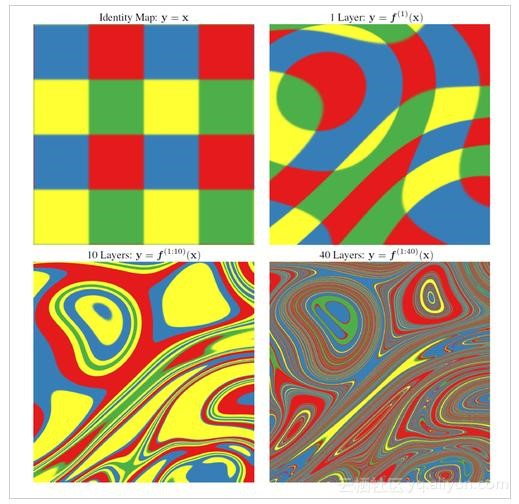
\includegraphics[width=1.0\textwidth]{figures/degradation1.jpg}
	\caption{权重矩阵的退化过程}
	\label{degradation1}
\end{figure}
\par 随着深度的增加,输入空间(左上角所示)会在输入空间中的每个点处被扭曲成越来越细的单丝,只有一个与细丝正交的方向影响网络的响应。沿着这个方向,网络实际上对变化变得非常敏感。

\subsection{预训练与微调(fine tuning)}
\subsubsection{深度网络存在问题}
\begin{itemize}
	\item 网络越深,需要的训练样本数越多。若用监督则需大量标注样本,不然小规模样本容易造成过拟合。深层网络特征比较多,会出现的多特征问题主要有多样本问题、规则化问题、特征选择问题。
	\item 多层神经网络参数优化是个高阶非凸优化问题,经常得到收敛较差的局部解
	\item 梯度扩散问题,BP算法计算出的梯度随着深度向前而显著下降,导致前面网络参数贡献很小,更新速度慢。
\end{itemize}
\subsubsection{解决方法}
逐层贪婪训练,无监督预训练(unsupervised pre-training)即训练网络的第一个隐藏层,再训练第二个…最后用这些训练好的网络参数值作为整体网络参数的初始值。经过预训练最终能得到比较好的局部最优解。
\subsubsection{模型微调fine tuning的定义}
用别人的参数、修改后的网络和自己的数据进行训练,使得参数适应自己的数据,这样一个过程,通常称之为微调(fine tuning)
\subsubsection{微调时网络参数的更新}
\begin{itemize}
	\item fine tune的过程相当于继续训练,跟直接训练的区别是初始化的时候。 
	\item 直接训练是按照网络定义指定的方式初始化。
	\item fine tune是用你已经有的参数文件来初始化。
\end{itemize}
\subsubsection{fine tuning模型的三种状态}
\begin{enumerate}
	\item 只预测,不训练:相对快、简单,针对那些已经训练好,现在要实际对未知数据进行标注的项目,非常高效。
	\item 训练,但只训练最后分类层:fine-tuning的模型最终的分类以及符合要求,现在只是在他们的基础上进行类别降维。
	\item 完全训练,分类层+之前卷积层都训练:跟状态二的差异很小,当然状态三比较耗时和需要训练GPU资源,不过非常适合fine-tuning到自己想要的模型里面,预测精度相比状态二也提高不少。
\end{enumerate}

\subsection{正则化Dropout}
\subsubsection{为什么要正则化}
深度学习可能存在过拟合问题——高方差,有两个解决方法,一个是正则化,另一个是准备更多的数据,这是非常可靠的方法,但你可能无法时时刻刻准备足够多的训练数据或者获取更多数据的成本很高,但正则化通常有助于避免过拟合或减少你的网络误差。 
\subsubsection{理解}
在每个训练批次中,通过忽略一半的特征检测器(让一半的隐层节点值为0),可以明显地减少过拟合现象。这种方式可以减少特征检测器(隐层节点)间的相互作用,检测器相互作用是指某些检测器依赖其他检测器才能发挥作用。Dropout说的简单一点就是:我们在前向传播的时候,让某个神经元的激活值以一定的概率p停止工作,这样可以使模型泛化性更强,因为它不会太依赖某些局部的特征。
\subsubsection{工作流程}
假设我们要训练这样一个神经网络,如图\ref{dropout1}所示。
\begin{figure}[htb]
	\centering
	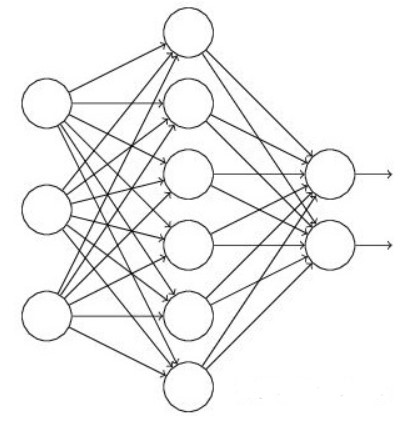
\includegraphics[width=0.6\textwidth]{figures/dropout1.jpg}
	\caption{正常的神经网络}
	\label{dropout1}
\end{figure}
\begin{enumerate}
	\item 首先随机(临时)删掉网络中一半的隐藏神经元,输入输出神经元保持不变(图\ref{dropout2}中虚线为部分临时被删除的神经元) \begin{figure}[htb]
		\centering
		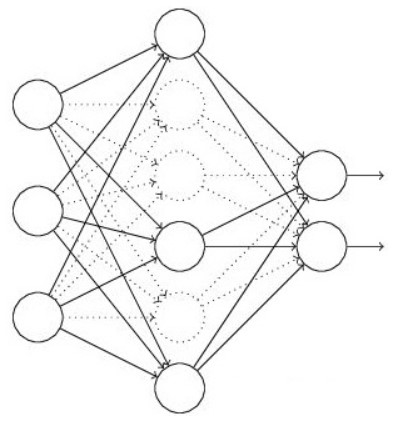
\includegraphics[width=0.6\textwidth]{figures/dropout2.jpg}
		\caption{删除部分神经元的神经网络}
		\label{dropout2}
	\end{figure}
	\item 然后把输入x通过修改后的网络前向传播,然后把得到的损失结果通过修改的网络反向传播。一小批训练样本执行完这个过程后,在没有被删除的神经元上按照随机梯度下降法更新对应的参数$(w, b)$
	\item 恢复被删掉的神经元(此时被删除的神经元保持原样,而没有被删除的神经元已经有所更新)
	\item 不断重复以上的过程。
\end{enumerate}
\subsubsection{工作机制}
\begin{enumerate}
	\item 取平均的作用: 先回到标准的模型即没有dropout,我们用相同的训练数据去训练5个不同的神经网络,一般会得到5个不同的结果,此时我们可以采用 “5个结果取均值”或者“多数取胜的投票策略”去决定最终结果。例如3个网络判断结果为数字9,那么很有可能真正的结果就是数字9,其它两个网络给出了错误结果。这种“综合起来取平均”的策略通常可以有效防止过拟合问题。因为不同的网络可能产生不同的过拟合,取平均则有可能让一些“相反的”拟合互相抵消。dropout掉不同的隐藏神经元就类似在训练不同的网络,随机删掉一半隐藏神经元导致网络结构已经不同,整个dropout过程就相当于对很多个不同的神经网络取平均。而不同的网络产生不同的过拟合,一些互为“反向”的拟合相互抵消就可以达到整体上减少过拟合。
	\item 减少神经元之间复杂的共适应关系: 因为dropout程序导致两个神经元不一定每次都在一个dropout网络中出现。这样权值的更新不再依赖于有固定关系的隐含节点的共同作用,阻止了某些特征仅仅在其它特定特征下才有效果的情况 。迫使网络去学习更加鲁棒的特征 ,这些特征在其它的神经元的随机子集中也存在。换句话说假如我们的神经网络是在做出某种预测,它不应该对一些特定的线索片段太过敏感,即使丢失特定的线索,它也应该可以从众多其它线索中学习一些共同的特征。从这个角度看dropout就有点像L1,L2正则,减少权重使得网络对丢失特定神经元连接的鲁棒性提高。
	\item Dropout类似于性别在生物进化中的角色:物种为了生存往往会倾向于适应这种环境,环境突变则会导致物种难以做出及时反应,性别的出现可以繁衍出适应新环境的变种,有效的阻止过拟合,即避免环境改变时物种可能面临的灭绝。
\end{enumerate}



\newpage
\section{卷积神经网络}
\subsection{特征选择}
\subsubsection{优化的常见问题}
在增加特征类别或者修改特征参数后:
\begin{itemize}
	\item 准确率提升不高
	\item 准确率不升反降
\end{itemize}
\subsubsection{理由}
\begin{itemize}
	\item 提取的特征中有冗余特征,对模型的性能几乎没有帮助。
	\item 提取的特征中有些可以列为噪声(或者可以称为老鼠屎),对模型的性能不仅没有帮助,还会降低模型的性能。
\end{itemize}
\subsubsection{本质}
是对一个给定特征子集的优良性通过一个特定的评价标准(evaluation criterion)进行衡量。
通过特征选择,原始特征集合中的冗余(redundant)特征和不相关(irrelevant)特征被除去。而有用特征得以保留。
\subsubsection{作用}
\begin{itemize}
	\item 降低了模型的复杂度,节省了大量计算资源以及计算时间。
	\item 提高了模型的泛化能力。
\end{itemize}
\subsubsection{具体方法}
考虑特征选择的策略的指标主要有两个:
\begin{itemize}
	\item 特征是否发散:如果一个特征不发散,就是说这个特征大家都有或者非常相似,说明这个特征不需要。
	\item 特征和目标是否相关:与目标的相关性越高,越应该优先选择。
\end{itemize}
总得来说,特征选择有三种常用的思路:
\begin{enumerate}
	\item 特征过滤(Filter Methods):对各个特征按照发散性或者相关 性进行评分,对分数设定阈值或者选择靠前得分的特征。\begin{itemize}
		\item 优点:简单,快。
		\item 缺点:对于排序靠前的特征,如果他们相关性较强,则引入了冗余特征,浪费了计算资源。 对于排序靠后的特征,虽然独立作用不显著,但和其他特征想组合可能会对模型有很好的帮助, 这样就损失了有价值的特征。
		\item 经典方法:皮尔逊相关系数(Pearson's Correlation),线性判别分析(Linear Discriminant Analysis,LDA),方差分析(Analysis of Variance,ANOVA),卡方检验(Chi-Square)。
	\end{itemize}
	\item 特征筛选(Wrapper Methods):通过不断排除特征或者不 断选择特征,并对训练得到的模型效果进行打分,通过预测 效果评 分来决定特征的去留。 \begin{itemize}
		\item 优点:能较好的保留有价值的特征。
		\item 缺点:会消耗巨大的计算资源和计算时间。
		\item 经典方法:前向选择法,后向剃除法,迭代剃除法
	\end{itemize}
	\item 嵌入法(Embedded Methods):有不少特征筛选和特征过滤的共性,主要的特点就是通过不同的方法去计算不同特征对于模型的贡献。\begin{itemize}
		\item 经典方法:Lasso,Elastic Net,Ridge Regression等。
	\end{itemize}
\end{enumerate}

\subsection{卷积}
\subsubsection{卷积公式}
$$\int_{-\infty}^{\infty}f(\tau)g(x-\tau)d\tau$$
\subsubsection{公式理解}
\begin{itemize}
	\item 系统某一时刻的输出是由多个输入共同作用(叠加)的结果。
	\item 所谓两个函数的卷积,本质上就是先将一个函数翻转,然后进行滑动叠加。
\end{itemize}
\subsubsection{例子:信号分析}
\par 如图\ref{signal1},输入信号是$f(t)$,是随时间变化的。系统响应函数是$g(t)$,图中的响应函数是随时间指数下降的,它的物理意义是说:如果在$t=0$的时刻有一个输入,那么随着时间的流逝,这个输入将不断衰减。换言之,到了$t=T$时刻,原来在$t=0$时刻的输入$f(0)$的值将衰减为$f(0)g(T)$。
\begin{figure}[htb]
	\centering
	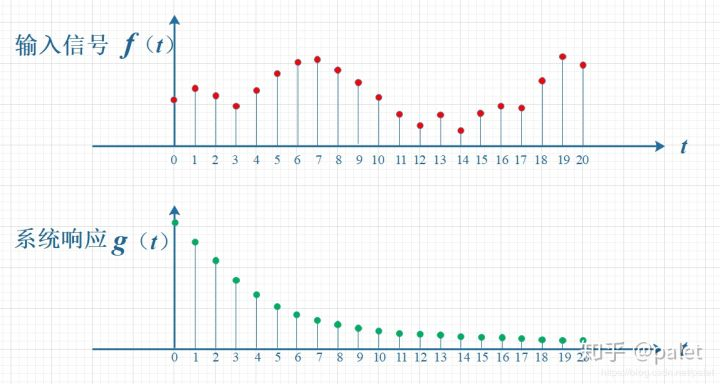
\includegraphics[width=0.80\textwidth]{figures/signal1.jpg}
	\caption{输入信号与系统响应}
	\label{signal1}
\end{figure}
\par 考虑到信号是连续输入的,也就是说,每个时刻都有新的信号进来,所以,最终输出的是所有之前输入信号的累积效果。
\par 如图\ref{signal2},在$t=T$时刻的输出信号为所有输入信号和其系统响应的乘积的和,但是可以看到,此时输入信号和系统响应的对应关系是相反的。
\begin{figure}[htb]
	\centering
	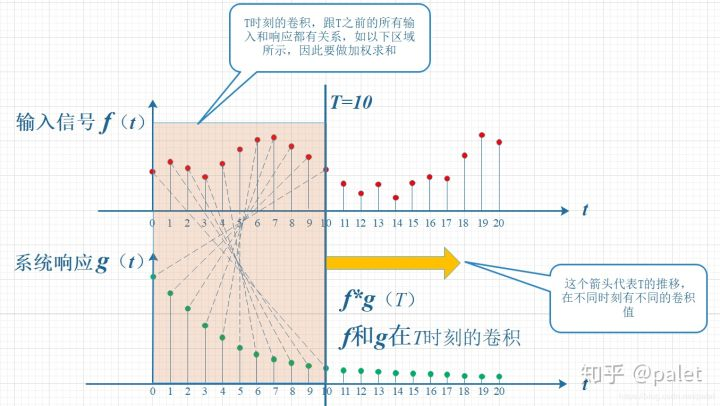
\includegraphics[width=0.80\textwidth]{figures/signal2.jpg}
	\caption{输入信号与系统响应的对应关系}
	\label{signal2}
\end{figure}
\par 所以我们对系统响应函数$g(t)$进行翻转,这样输入信号和系统响应的对应关系就是顺着的了。如图\ref{signal3}所示。
\begin{figure}[htb]
	\centering
	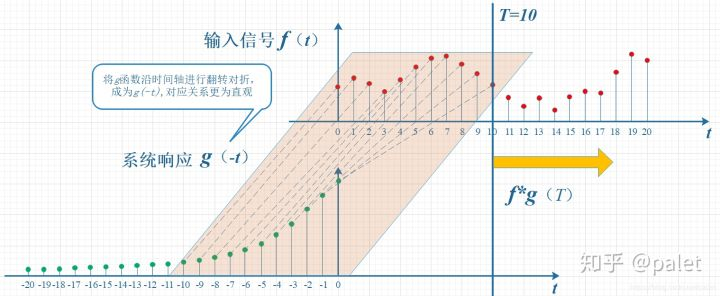
\includegraphics[width=0.80\textwidth]{figures/signal3.jpg}
	\caption{输入信号与翻转后的系统响应}
	\label{signal3}
\end{figure}
\par 最后我们再对$g(t)$加上$T$,将其和输入信号对齐。如图\ref{signal4}所示。
\begin{figure}[htb]
	\centering
	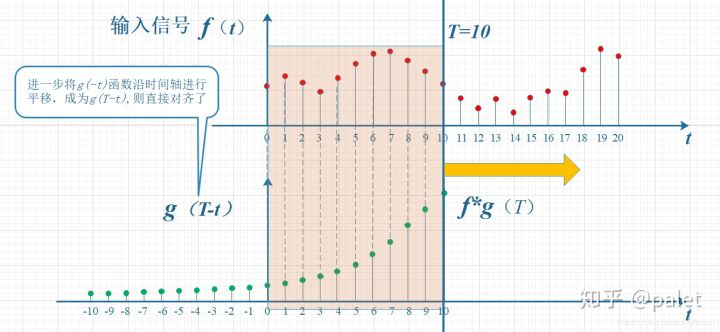
\includegraphics[width=0.80\textwidth]{figures/signal4.jpg}
	\caption{输入信号与最终的系统响应}
	\label{signal4}
\end{figure}

\subsection{卷积神经网络的结构}
\begin{table}[h!]
	\begin{tabular}{|p{100pt}|p{100pt}|p{100pt}|}
		\hline
		卷积层 & 采样层 & 全连接层 \\
		\hline
		提取图片特征 & 保留我们想要的或者重要的特征 & 模仿人脑进行判断 \\
		\hline
	\end{tabular}
\end{table}
\subsubsection{全连接层}
假如我们想要让机器识别一个图片数字2,那么我们就需要一个类似人脑的构造来进行识别,这就是全连接层。假设全连接层为三层的神经元个数分别为1024,512,10.
\par 但是假设图片大小为$32*32$,那么我们全连接层的参数个数为$3*32*32*1024+1024*512+512*10+1024(bias)+512(bias)=3676672$个。参数太多会导致训练时间过长,还有可能会导致过拟合。
\begin{figure}[htb]
	\centering
	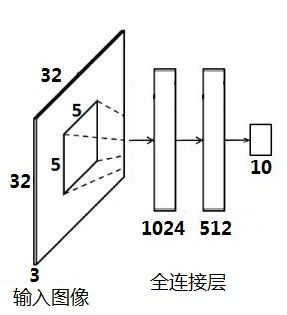
\includegraphics[width=0.50\textwidth]{figures/cnn1.jpg}
	\caption{只有全连接层的CNN}
	\label{cnn1}
\end{figure}
\subsubsection{采样层}
为了解决全连接层参数过多的问题,我们希望主要提取图像的边缘特征,对于灰色和黑色这种冗余或者不重要的的区域特征,我们尽量丢弃或者少保留,那么这样可能会减少参数或者减少提参数的过程。
\par 此时采样层应运而生。
\begin{figure}[htb]
	\centering
	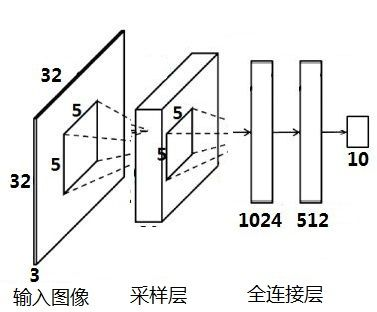
\includegraphics[width=0.50\textwidth]{figures/cnn2.jpg}
	\caption{加入采样层的CNN}
	\label{cnn2}
\end{figure}
\subsubsection{卷积层}
首先将图片进行分解,在顺序不变的情况下我们还是可以识别出内容是2.
但是我们如果将分解后的子图的顺序进行交换,那就无法识别出数字2.
\begin{figure}[htb]
	\centering
	\begin{minipage}[htb]{0.3\textwidth}
		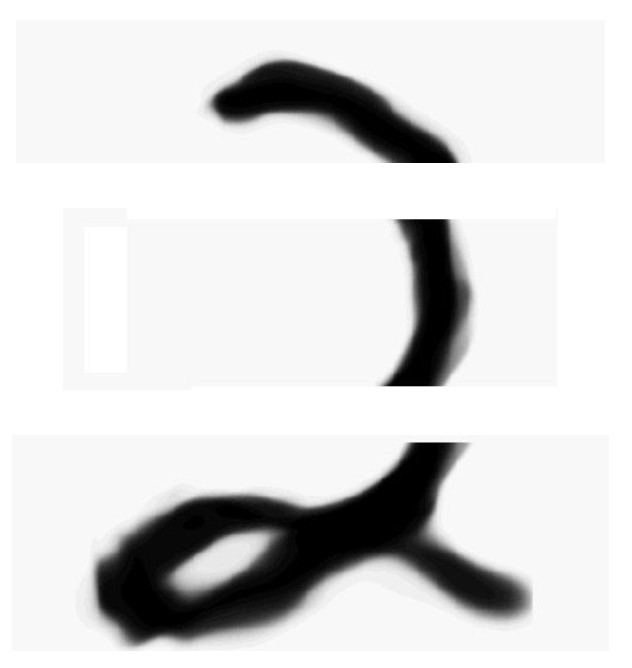
\includegraphics[width=0.80\textwidth]{figures/cnn3.jpg}
		\caption{顺序不变的子图}
		\label{cnn3}
	\end{minipage}
	\begin{minipage}[htb]{0.3\textwidth}
		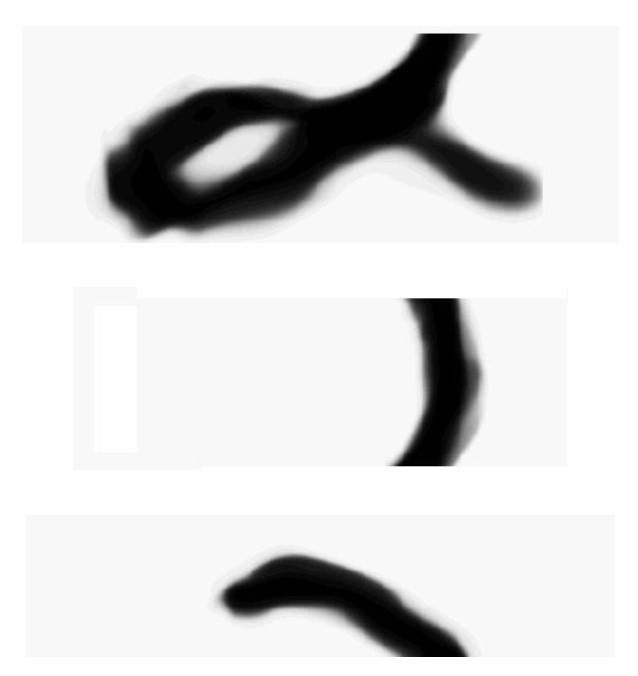
\includegraphics[width=0.80\textwidth]{figures/cnn4.jpg}
		\caption{顺序改变的子图}
		\label{cnn4}
	\end{minipage}
\end{figure}
由此我们可以得出:
\begin{itemize}
	\item 如果我们只知道局部的图片,以及局部的相对位置,只要我们能将它正确组合起来,我们也可以对物体进行识别
	\item 局部与局部之间关联性不大,也就是局部的变化,很少影响到另外一个局部
\end{itemize}
同时还有两个问题需要解决:
\begin{itemize}
	\item 输入的只是原始图片,我们还没有提取图片的特征
	\item 我们目前要处理的参数仍然非常多,我们需要对原始输入进行降维或者减少参数
\end{itemize}
此时我们加入卷积层,一方面提取特征,另一方面减少参数个数。
\begin{figure}[htb]
	\centering
	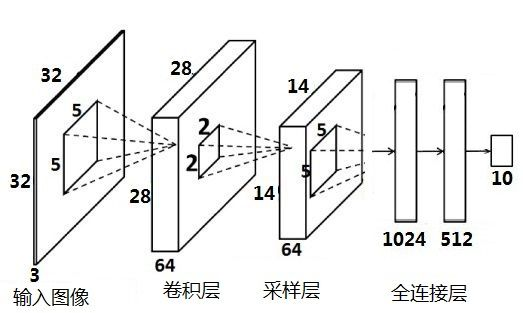
\includegraphics[width=0.6\textwidth]{figures/cnn5.jpg}
	\caption{卷积层的CNN}
	\label{cnn5}
\end{figure}
\subsubsection{级联分类器}
除此之外,我们还会遇到两个问题:
\begin{itemize}
	\item 卷积层提取的特征数量有限,无法提取图片全部特征
	\item 无法确定采样层选取的特征是否重要
\end{itemize}
\par 此时我们需要一个级联分类器。
\par 大概意思就是我从一堆弱分类器里面,挑出一个最符合要求的弱分类器,用着这个弱分类器把不想要的数据剔除,保留想要的数据
然后再从剩下的弱分类器里,再挑出一个最符合要求的弱分类器,对上一级保留的数据,把不想要的数据剔除,保留想要的数据。
最后,通过不断串联几个弱分类器,进过数据层层筛选,最后得到我们想要的数据。
\begin{figure}[htb]
	\centering
	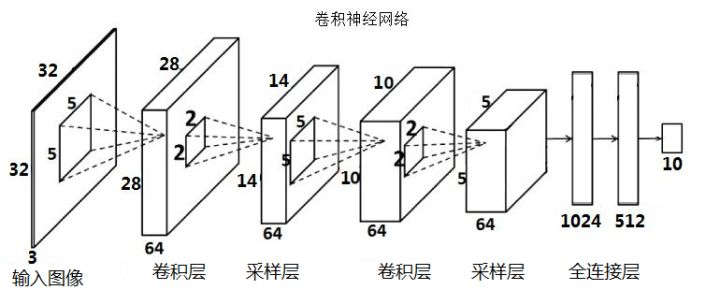
\includegraphics[width=0.6\textwidth]{figures/cnn6.jpg}
	\caption{级联分类器的CNN}
	\label{cnn6}
\end{figure}

\subsection{卷积层:提取特征}
\subsubsection{图示}
\begin{figure}[htb]
	\centering
	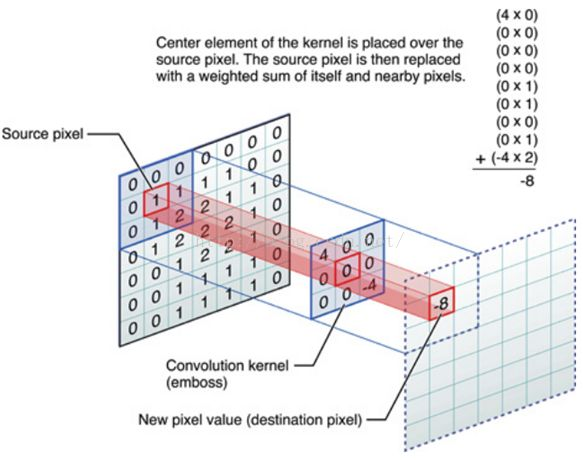
\includegraphics[width=0.6\textwidth]{figures/convolution1.jpg}
	\caption{卷积核的卷积过程}
	\label{convolution1}
\end{figure}
\begin{itemize}
	\item 卷积核放在神经网络里,就代表对应的权重(weight)
	\item 卷积核和图像进行点乘(dot product), 就代表卷积核里的权重单独对相应位置的Pixel进行作用
\end{itemize}
\subsubsection{输出}
根据神经网络公式:
$$\sum_i \omega_ix_i + b$$
在此,我们先假设$b=0$,而最终的输出$FinalOutput = \sum_ioutput_{\omega_i} + b$
\subsubsection{卷积顺序}
除此之外,我们还需要决定卷积的顺序:从左到右,每隔x列Pixel,向右移动一次卷积核进行卷积(x可以自己定义),其中x叫作stride,就是步长的意思,如果我们$x = 2$, 就是相当每隔两行或者两列进行卷积
\begin{figure}[htb]
	\centering
	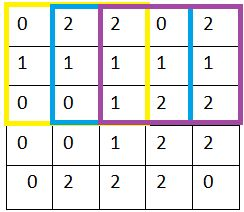
\includegraphics[width=0.3\textwidth]{figures/sequence1.jpg}
	\caption{卷积顺序(x=1)}
	\label{sequence1}
\end{figure}
\subsubsection{补0}
\begin{figure}[htb]
	\centering
	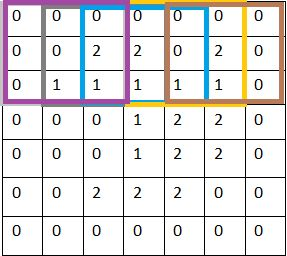
\includegraphics[width=0.5\textwidth]{figures/zeropadding1.jpg}
	\caption{补0}
	\label{zeropadding1}
\end{figure}
\paragraph{作用}
同样是stride x=1 的情况下,补0比原来没有添0 的情况下进行卷积,从左到右,从上到下都多赚了2次卷积,这样第一层卷积层输出的特征图(feature map)仍然为5x5,和输入图片的大小一致。
\paragraph{好处}
\begin{itemize}
	\item 获得的更多更细致的特征信息,可以获得更多的图像边缘信息
	\item 可以控制卷积层输出的特征图的size,从而可以达到控制网络结构的作用,还是以上面的例子,如果没有做zero-padding以及第二层卷积层的卷积核仍然是3x3, 那么第二层卷积层输出的特征图就是1x1,CNN的特征提取就这么结束了。
\end{itemize}

\subsection{采样层:特征选择}
\subsubsection{示例:Maxpooling}
首先假设卷积层获得的特征值矩阵如图\ref{maxpooling1}所示。
\begin{figure}[htb]
	\centering
	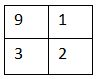
\includegraphics[width=0.3\textwidth]{figures/maxpooling1.jpg}
	\caption{特征值矩阵}
	\label{maxpooling1}
\end{figure}
\par 而Maxpooling实际上为从矩阵中选择最大的值:此处即为9。如图\ref{maxpooling2}所示。
\begin{figure}[htb]
	\centering
	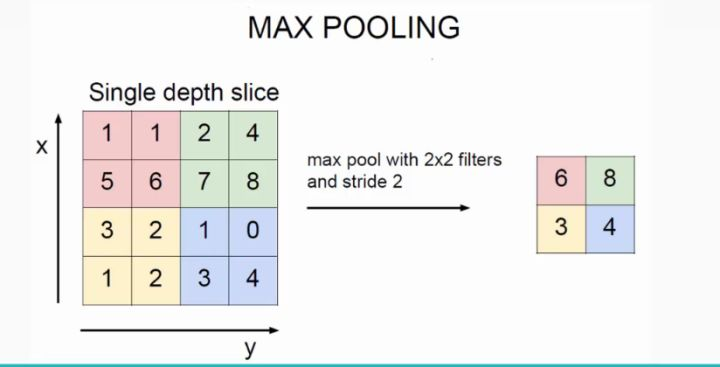
\includegraphics[width=1.0\textwidth]{figures/maxpooling2.jpg}
	\caption{Maxpooling}
	\label{maxpooling2}
\end{figure}
\subsubsection{好处}
\begin{itemize}
	\item 避免过拟合
	\item 避免参数过多导致的训练代价太大
	\item 无法满足模型的结构需求
\end{itemize}
\subsubsection{性质}
采样层还有一定程度的空间不变性。图像经过一个小小的平移之后,依然产生相同的池化特征。

\subsection{全连接层:进行分类}
\subsubsection{图示}
\begin{figure}[htb]
	\centering
	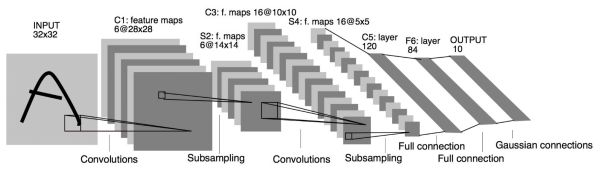
\includegraphics[width=1.0\textwidth]{figures/fullconnector1.jpg}
	\caption{带有全连接层的CNN结构}
	\label{fullconnector1}
\end{figure}
\subsubsection{转化方法}
因为采样层所提取的特征一般都是$n*n*c$的,其中$c$是filter的个数。而全连接层是一个普通的神经网络,每一层是由许多神经元组成的$(1*4096)$的平铺结构。那么如何将$n*n*c$转化成$1*4096$就是需要解决的问题。
\par 此时采用的方法是进行一次“卷积”。用一个3x3x5的filter 去卷积激活函数的输出,得到的结果就是一个fully connected layer 的一个神经元的输出,这个输出就是一个值。因为我们有4096个神经元,我们实际就是用一个3x3x5x4096的卷积层去卷积激活函数的输出。如图\ref{fullconnector2}所示。
\begin{figure}[htb]
	\centering
	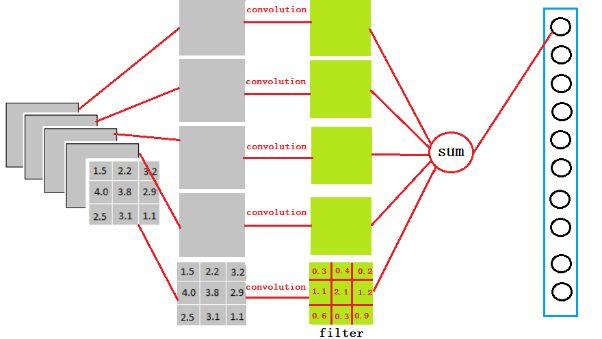
\includegraphics[width=0.8\textwidth]{figures/fullconnector2.jpg}
	\caption{“卷积”操作}
	\label{fullconnector2}
\end{figure}
\subsubsection{作用}
把特征representation整合到一起,输出为一个值。可以大大减少特征位置对分类带来的影响。
\subsubsection{对模型的影响因素}
\begin{itemize}
	\item 全接解层的总层数(长度)
	\item 单个全连接层的神经元数(宽度)
	\item 激活函数
\end{itemize}

\subsection{局部响应归一化作用}
LRN 是一种提高深度学习准确度的技术方法。LRN一般是在激活、池化函数后的一种方法。
\par 在ALexNet中,提出了LRN层,对局部神经元的活动创建竞争机制,使其中响应比较大对值变得相对更大,并抑制其他反馈较小的神经元,增强了模型的泛化能力。
\subsubsection{理解局部响应归一化}
局部响应归一化原理是仿造生物学上活跃的神经元对相邻神经元的抑制现象(侧抑制),其公式如下:
$$b_{x,y}^i = a_{x,y}^i / (k + \alpha \sum_{j=max(0, i-n/2)}^{min(N-1, i+n/2)}(a_{x,y}^j)^2 )^\beta$$
\begin{itemize}
	\item $a$:表示卷积层(包括卷积操作和池化操作)后的输出结果,是一个四维数组[batch,height,width,channel]。 \begin{enumerate}
		\item batch:批次数(每一批为一张图片)。
		\item height:图片高度。
		\item width:图片宽度。
		\item channel:通道数。可以理解成一批图片中的某一个图片经过卷积操作后输出的神经元个数,或理解为处理后的图片深度。
	\end{enumerate}
	\item $ a_{x,y}^i $表示在这个输出结构中的一个位置$ [a,b,c,d] $,可以理解成在某一张图中的某一个通道下的某个高度和某个宽度位置的点,即第$ a $张图的第$ d $个通道下的高度为b宽度为c的点。
	\item $ N $:论文公式中的$ N $表示通道数 (channel)。
	\item $ a $,$ n/2 $,$ k $分别表示函数中的input,depth radius,bias。参数$ k, n, \alpha, \beta $都是超参数,一般设置$ k=2, n=5, \alpha=1*e-4, \beta=0.75 $
	\item $ \sum $:$ \sum $叠加的方向是沿着通道方向的,即每个点值的平方和是沿着$ a $中的第3维channel方向的,也就是一个点同方向的前面$ n/2 $个通道(最小为第$ 0 $个通道)和后$ n/2 $个通道(最大为第$ d-1 $个通道)的点的平方和(共$ n+1 $个点)。而函数的英文注解中也说明了把input当成是$ d $个3维的矩阵,说白了就是把input的通道数当作3维矩阵的个数,叠加的方向也是在通道方向。 
\end{itemize}
如图\ref{LRN1}所示。
\begin{figure}[htb]
	\centering
	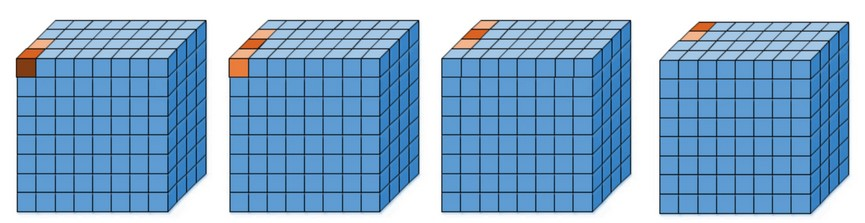
\includegraphics[width=0.8\textwidth]{figures/LRN1.jpg}
	\caption{LRN}
	\label{LRN1}
\end{figure}
\subsubsection{实例}
假设存在一LRN如图\ref{LRN2}所示。
\begin{figure}[htb]
	\centering
	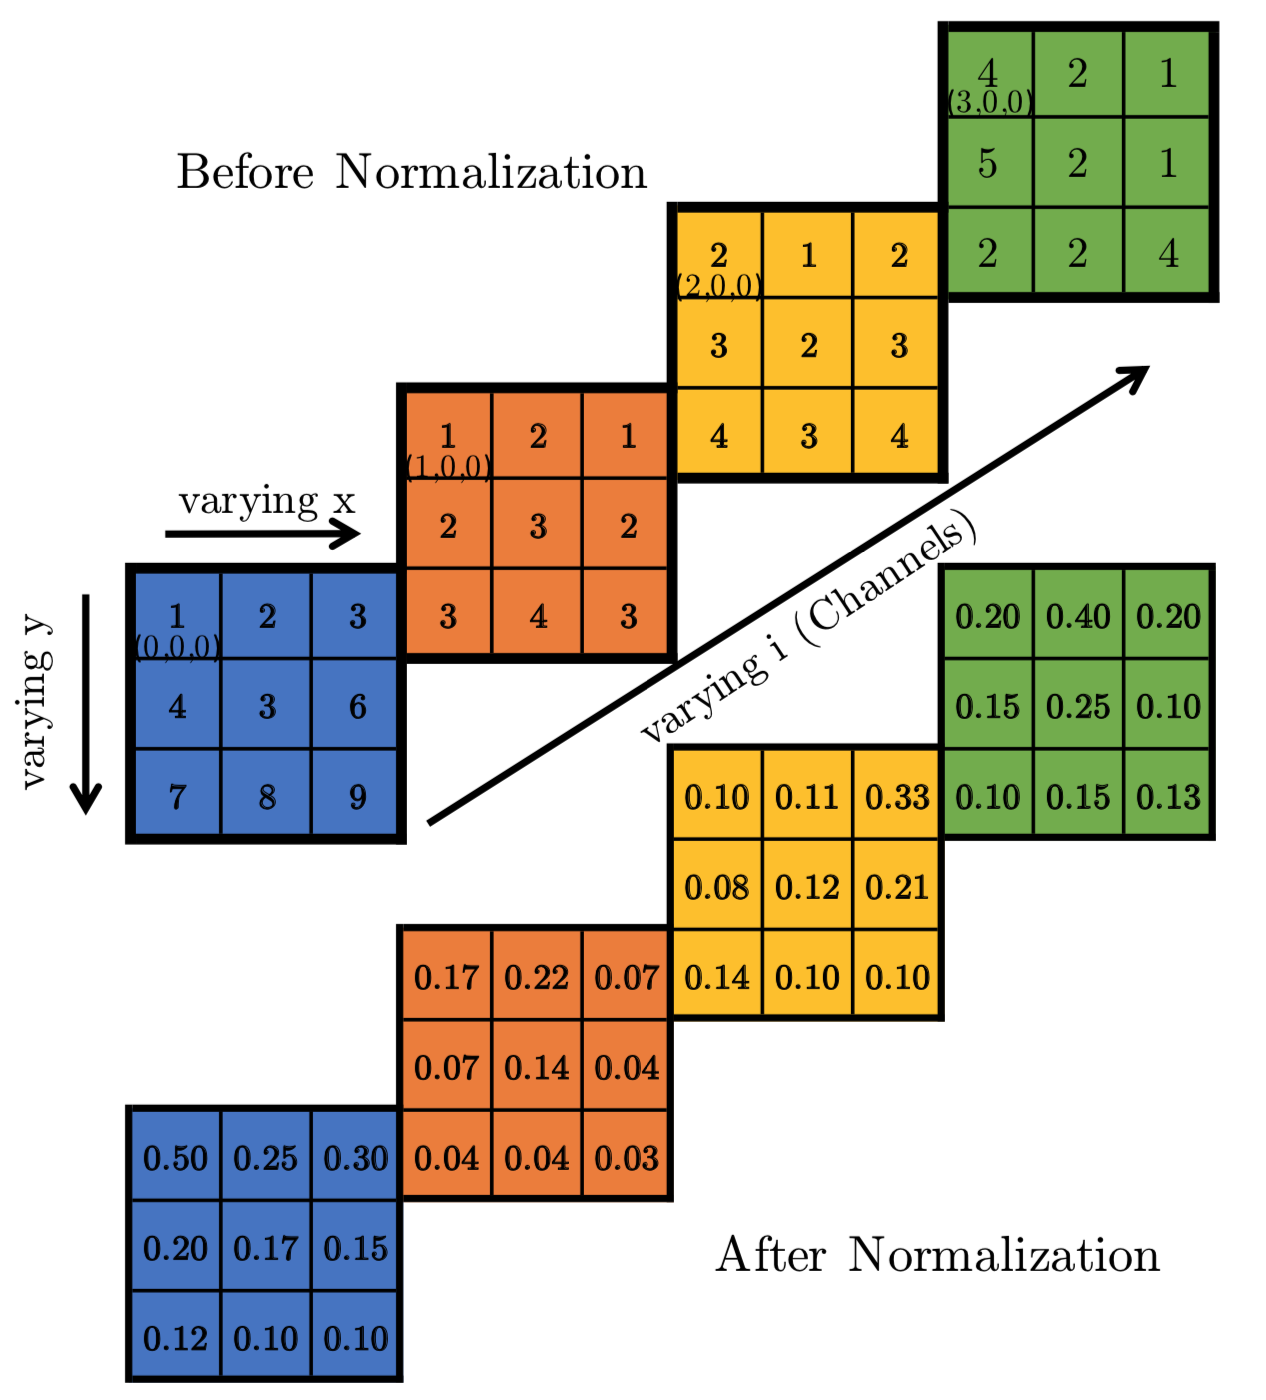
\includegraphics[width=0.8\textwidth]{figures/LRN2.png}
	\caption{LRN}
	\label{LRN2}
\end{figure}
\par 不同的颜色表示不同的通道,因此N=4。
令超参数$(k,\alpha,\beta,n) = (0, 1, 1, 2)$。
$n=2$的值表示在计算位置$(i,x,y)$处的归一化值时,我们考虑上一个过滤器和下一个过滤器相同位置的值:$(i-1, x, y)$和$(i + 1, x, y)$。
例如对于$(i, x, y) =(0, 0, 0)$,我们有值$(i, x, y) = 1$,而值$(i-1,x, y)$不存在,值$(i +1, x, y) = 1$。因此$Normalized value (i, x, y) = 1 /(1²+ 1²) = 0.5$。
可以看到上图的下部。其余的归一化值以类似的方式计算。

\subsection{批归一化BN}
以前在神经网络训练中,只是对输入层数据进行归一化处理,却没有在中间层进行归一化处理。要知道,虽然我们对输入数据进行了归一化处理,但是输入数据经过 $ \sigma(WX+b) $ 这样的矩阵乘法以及非线性运算之后,其数据分布很可能被改变,而随着深度网络的多层运算之后,数据分布的变化将越来越大。如果我们能在网络的中间也进行归一化处理,是否对网络的训练起到改进作用呢?答案是肯定的。 
这种在神经网络中间层也进行归一化处理,使训练效果更好的方法,就是批归一化Batch Normalization(BN)。
\subsubsection{优点}
\begin{itemize}
	\item 减少了人为选择参数。在某些情况下可以取消dropout和L2正则项参数,或者采取更小的L2正则项约束参数;
	\item 减少了对学习率的要求。现在我们可以使用初始很大的学习率或者选择了较小的学习率,算法也能够快速训练收敛;
	\item 可以不再使用局部响应归一化。BN本身就是归一化网络(局部响应归一化在AlexNet网络中存在) 
	\item 破坏原来的数据分布,一定程度上缓解过拟合(防止每批训练中某一个样本经常被挑选到,文献说这个可以提高1\%的精度)。 
	\item 减少梯度消失,加快收敛速度,提高训练精度。
\end{itemize}
\subsubsection{算法流程}
输入:上一层输出结果 $ X = {x_1, x_2, ..., x_m} $,学习参数 $ \gamma, \beta $
\begin{enumerate}
	\item 计算上一层输出数据的均值: $$\mu_{\beta} = \frac{1}{m} \sum_{i=1}^m(x_i)$$ 其中,$ m $是此次训练样本batch的大小。
	\item 计算上一层输出数据的标准差: $$\sigma_{\beta}^2 = \frac{1}{m} \sum_{i=1}^m (x_i - \mu_{\beta})^2$$ 
	\item 归一化处理,得到: $$\hat x_i = \frac{x_i + \mu_{\beta}}{\sqrt{\sigma_{\beta}^2 + \epsilon}}$$ 其中$ \epsilon $是为了避免分母为0而加进去的接近于0的很小值
	\item 重构,对经过上面归一化处理得到的数据进行重构,得到: $$y_i = \gamma \hat x_i + \beta$$  其中,$ \gamma, \beta $为可学习参数。
\end{enumerate}
\par 上述是BN训练时的过程,但是当在投入使用时,往往只是输入一个样本,没有所谓的均值$ \mu_{\beta} $和标准差$ \sigma_{\beta}^2 $。
此时,均值$ \mu_{\beta} $是计算所有batch$ \mu_{\beta} $值的平均值得到,标准差$ \sigma_{\beta}^2 $采用每个batch$ \sigma_{\beta}^2 $的无偏估计得到。
\par 除此以外,$\gamma$和$\beta$分别是用来控制平均值和方差的参数。

\newpage
\subsection{生成对抗网络}
\begin{algorithm}[htb]  
	\caption{Mini-batch随机梯度下降算法。其中k为超参数,代表着判别器所需的步骤数。此处为了减轻训练负担,取k=1}  
	\begin{algorithmic}[1]  	  
	\For{训练迭代次数}
		\For{k步}
			\State 从之前的噪声$p_g (z)$中取出minibatch所需的m个噪声样例$\{z^{(1)},...,z^{(m)} \}$
			\State 从数据生成分布$p_{data}(x)$中取出minibatch所需的m个数据样例$\{x^{(1)},...,x^{(m)} \}$
			\State 通过随机梯度下降算法更新判别器参数:$$\nabla_{\theta_d} \frac{1}{m} \sum_{i=1}^m [\log D(x^{(i)}) + \log (1-D(G(z^{(i)})))] $$
		\EndFor
		\State 从之前的噪声$p_g (z)$中取出minibatch所需的m个噪声样例$\{z^{(1)},...,z^{(m)} \}$
		\State 通过随机梯度下降算法更新生成器参数:$$\nabla_{\theta_d} \frac{1}{m} \sum_{i=1}^m \log (1-D(G(z^{(i)})))$$
	\EndFor
	\\
	基于梯度的更新可以使用任何标准的基于梯度的学习规则。此处使用的是momentum算法。
    \end{algorithmic}   
\end{algorithm}  

\begin{algorithm}[htb]  
	\caption{WGAN,以下参数中:$\alpha=0.00005,c=0.01,m=64,n_{critic}=5$}  
	\begin{algorithmic}[1]
		\Require  
		学习率$\alpha$,截断常数c,批大小m,生成器每次迭代的迭代数量$n_{critic}$  
	  	\Require  
	  	起始critic参数值$\omega_0$,初始生成器参数值$\theta_0$  	  
	\While{$\theta$没有收敛}
		\For{$t=0,...,n_{critic}$}
			\State 从真实数据$P_r$中取出所需的m个数据样例$\{x^{(1)},...,x^{(m)} \}$
			\State 从之前的样例$p(z)$中取出所需的m个样例$\{z^{(1)},...,z^{(m)} \}$
			\State $g_{\omega} \gets \nabla_\omega [\frac{1}{m}\sum_{i=1}^m f_\omega(x^{(i)})-\frac{1}{m}\sum_{i=1}^m f_\omega(g_\theta (z^{(i)}))]$
			\State $\omega \gets \omega + \alpha \cdot RMSProp(\omega,g_\omega)$
			\State $\omega \gets clip(\omega, -c, c)$
		\EndFor
		\State 从之前的样例$p_g (z)$中取出所需的m个样例$\{z^{(1)},...,z^{(m)} \}$
		\State $g_{\theta} \gets \nabla_\theta \frac{1}{m}\sum_{i=1}^m f_\omega(g_\theta (z^{(i)}))$
		\State $\theta \gets \theta + \alpha \cdot RMSProp(\theta,g_\theta)$
	\EndWhile
	\end{algorithmic}   
\end{algorithm}  

\end{document}